\documentclass[conference]{IEEEtran}
% Some very useful LaTeX packages include:
% (uncomment the ones you want to load)

\usepackage{balance}
\usepackage{booktabs}
\usepackage{enumerate}
% *** MISC UTILITY PACKAGES ***
%
%\usepackage{ifpdf}
% Heiko Oberdiek's ifpdf.sty is very useful if you need conditional
% compilation based on whether the output is pdf or dvi.
% usage:
% \ifpdf
%   % pdf code
% \else
%   % dvi code
% \fi
% The latest version of ifpdf.sty can be obtained from:
% http://www.ctan.org/pkg/ifpdf
% Also, note that IEEEtran.cls V1.7 and later provides a builtin
% \ifCLASSINFOpdf conditional that works the same way.
% When switching from latex to pdflatex and vice-versa, the compiler may
% have to be run twice to clear warning/error messages.

% *** CITATION PACKAGES ***
%
%\usepackage{cite}
% cite.sty was written by Donald Arseneau
% V1.6 and later of IEEEtran pre-defines the format of the cite.sty package
% \cite{} output to follow that of the IEEE. Loading the cite package will
% result in citation numbers being automatically sorted and properly
% "compressed/ranged". e.g., [1], [9], [2], [7], [5], [6] without using
% cite.sty will become [1], [2], [5]--[7], [9] using cite.sty. cite.sty's
% \cite will automatically add leading space, if needed. Use cite.sty's
% noadjust option (cite.sty V3.8 and later) if you want to turn this off
% such as if a citation ever needs to be enclosed in parenthesis.
% cite.sty is already installed on most LaTeX systems. Be sure and use
% version 5.0 (2009-03-20) and later if using hyperref.sty.
% The latest version can be obtained at:
% http://www.ctan.org/pkg/cite
% The documentation is contained in the cite.sty file itself.


% *** GRAPHICS RELATED PACKAGES ***
%
\ifCLASSINFOpdf
   \usepackage[pdftex]{graphicx}
  % declare the path(s) where your graphic files are
   \graphicspath{{../pdf/}{../jpeg/}}
  % and their extensions so you won't have to specify these with
  % every instance of \includegraphics
  % \DeclareGraphicsExtensions{.pdf,.jpeg,.png}
\else
  % or other class option (dvipsone, dvipdf, if not using dvips). graphicx
  % will default to the driver specified in the system graphics.cfg if no
  % driver is specified.
   \usepackage[dvips]{graphicx}
  % declare the path(s) where your graphic files are
   \graphicspath{{../eps/}}
  % and their extensions so you won't have to specify these with
  % every instance of \includegraphics
  % \DeclareGraphicsExtensions{.eps}
\fi
% graphicx was written by David Carlisle and Sebastian Rahtz. It is
% required if you want graphics, photos, etc. graphicx.sty is already
% installed on most LaTeX systems. The latest version and documentation
% can be obtained at: 
% http://www.ctan.org/pkg/graphicx
% Another good source of documentation is "Using Imported Graphics in
% LaTeX2e" by Keith Reckdahl which can be found at:
% http://www.ctan.org/pkg/epslatex
%
% latex, and pdflatex in dvi mode, support graphics in encapsulated
% postscript (.eps) format. pdflatex in pdf mode supports graphics
% in .pdf, .jpeg, .png and .mps (metapost) formats. Users should ensure
% that all non-photo figures use a vector format (.eps, .pdf, .mps) and
% not a bitmapped formats (.jpeg, .png). The IEEE frowns on bitmapped formats
% which can result in "jaggedy"/blurry rendering of lines and letters as
% well as large increases in file sizes.
%
% You can find documentation about the pdfTeX application at:
% http://www.tug.org/applications/pdftex

% *** MATH PACKAGES ***
%
%\usepackage{amsmath}
% A popular package from the American Mathematical Society that provides
% many useful and powerful commands for dealing with mathematics.
%
% Note that the amsmath package sets \interdisplaylinepenalty to 10000
% thus preventing page breaks from occurring within multiline equations. Use:
%\interdisplaylinepenalty=2500
% after loading amsmath to restore such page breaks as IEEEtran.cls normally
% does. amsmath.sty is already installed on most LaTeX systems. The latest
% version and documentation can be obtained at:
% http://www.ctan.org/pkg/amsmath

% *** SPECIALIZED LIST PACKAGES ***
%
%\usepackage{algorithmic}
% algorithmic.sty was written by Peter Williams and Rogerio Brito.
% This package provides an algorithmic environment fo describing algorithms.
% You can use the algorithmic environment in-text or within a figure
% environment to provide for a floating algorithm. Do NOT use the algorithm
% floating environment provided by algorithm.sty (by the same authors) or
% algorithm2e.sty (by Christophe Fiorio) as the IEEE does not use dedicated
% algorithm float types and packages that provide these will not provide
% correct IEEE style captions. The latest version and documentation of
% algorithmic.sty can be obtained at:
% http://www.ctan.org/pkg/algorithms
% Also of interest may be the (relatively newer and more customizable)
% algorithmicx.sty package by Szasz Janos:
% http://www.ctan.org/pkg/algorithmicx

% *** ALIGNMENT PACKAGES ***
%
%\usepackage{array}
% Frank Mittelbach's and David Carlisle's array.sty patches and improves
% the standard LaTeX2e array and tabular environments to provide better
% appearance and additional user controls. As the default LaTeX2e table
% generation code is lacking to the point of almost being broken with
% respect to the quality of the end results, all users are strongly
% advised to use an enhanced (at the very least that provided by array.sty)
% set of table tools. array.sty is already installed on most systems. The
% latest version and documentation can be obtained at:
% http://www.ctan.org/pkg/array


% IEEEtran contains the IEEEeqnarray family of commands that can be used to
% generate multiline equations as well as matrices, tables, etc., of high
% quality.

% *** SUBFIGURE PACKAGES ***

% subfig.sty, written by Steven Douglas Cochran, is the modern replacement
% for subfigure.sty, the latter of which is no longer maintained and is
% incompatible with some LaTeX packages including fixltx2e. However,
% subfig.sty requires and automatically loads Axel Sommerfeldt's caption.sty
% which will override IEEEtran.cls' handling of captions and this will result
% in non-IEEE style figure/table captions. To prevent this problem, be sure
% and invoke subfig.sty's "caption=false" package option (available since
% subfig.sty version 1.3, 2005/06/28) as this is will preserve IEEEtran.cls
% handling of captions.
% Note that the Computer Society format requires a larger sans serif font
% than the serif footnote size font used in traditional IEEE formatting
% and thus the need to invoke different subfig.sty package options depending
% on whether compsoc mode has been enabled.
%
% The latest version and documentation of subfig.sty can be obtained at:
% http://www.ctan.org/pkg/subfig

% *** FLOAT PACKAGES ***
%
%\usepackage{fixltx2e}
% fixltx2e, the successor to the earlier fix2col.sty, was written by
% Frank Mittelbach and David Carlisle. This package corrects a few problems
% in the LaTeX2e kernel, the most notable of which is that in current
% LaTeX2e releases, the ordering of single and double column floats is not
% guaranteed to be preserved. Thus, an unpatched LaTeX2e can allow a
% single column figure to be placed prior to an earlier double column
% figure.
% Be aware that LaTeX2e kernels dated 2015 and later have fixltx2e.sty's
% corrections already built into the system in which case a warning will
% be issued if an attempt is made to load fixltx2e.sty as it is no longer
% needed.
% The latest version and documentation can be found at:
% http://www.ctan.org/pkg/fixltx2e


%\usepackage{stfloats}
% stfloats.sty was written by Sigitas Tolusis. This package gives LaTeX2e
% the ability to do double column floats at the bottom of the page as well
% as the top. (e.g., "\begin{figure*}[!b]" is not normally possible in
% LaTeX2e). It also provides a command:
%\fnbelowfloat
% to enable the placement of footnotes below bottom floats (the standard
% LaTeX2e kernel puts them above bottom floats). This is an invasive package
% which rewrites many portions of the LaTeX2e float routines. It may not work
% with other packages that modify the LaTeX2e float routines. The latest
% version and documentation can be obtained at:
% http://www.ctan.org/pkg/stfloats
% Do not use the stfloats baselinefloat ability as the IEEE does not allow
% \baselineskip to stretch. Authors submitting work to the IEEE should note
% that the IEEE rarely uses double column equations and that authors should try
% to avoid such use. Do not be tempted to use the cuted.sty or midfloat.sty
% packages (also by Sigitas Tolusis) as the IEEE does not format its papers in
% such ways.
% Do not attempt to use stfloats with fixltx2e as they are incompatible.
% Instead, use Morten Hogholm'a dblfloatfix which combines the features
% of both fixltx2e and stfloats:
%
% \usepackage{dblfloatfix}
% The latest version can be found at:
% http://www.ctan.org/pkg/dblfloatfix

% *** PDF, URL AND HYPERLINK PACKAGES ***
%
%\usepackage{url}
% url.sty was written by Donald Arseneau. It provides better support for
% handling and breaking URLs. url.sty is already installed on most LaTeX
% systems. The latest version and documentation can be obtained at:
% http://www.ctan.org/pkg/url
% Basically, \url{my_url_here}.


% *** Do not adjust lengths that control margins, column widths, etc. ***
% *** Do not use packages that alter fonts (such as pslatex).         ***
% There should be no need to do such things with IEEEtran.cls V1.6 and later.
% (Unless specifically asked to do so by the journal or conference you plan
% to submit to, of course. )


% correct bad hyphenation here
\hyphenation{op-tical net-works semi-conduc-tor}
\usepackage[spanish]{babel}
\selectlanguage{spanish}
\usepackage[utf8]{inputenc}

\renewcommand{\labelitemi}{$\bullet$} 

%\usepackage{caption}% http://ctan.org/pkg/caption
\ifCLASSOPTIONcompsoc
  \usepackage[caption=false,font=normalsize,labelfont=sf,textfont=sf,justification=centering]{subfig}
\else
  \usepackage[caption=false,font=footnotesize,justification=centering]{subfig}
\fi

\captionsetup[table]{format=plain,labelformat=simple,labelsep=period,font={small,sc}, justification=centering}%


%\captionsetup[subfig]{caption=false,font=normalsize,labelfont=sf,textfont=sf,justification=centering}

\renewcommand\spanishtablename{\sc{Tabla}}

\begin{document}
\bstctlcite{IEEEexample:BSTcontrol}
%
% paper title
% Titles are generally capitalized except for words such as a, an, and, as,
% at, but, by, for, in, nor, of, on, or, the, to and up, which are usually
% not capitalized unless they are the first or last word of the title.
% Linebreaks \\ can be used within to get better formatting as desired.
% Do not put math or special symbols in the title.
\title{Juegos de Entrenamiento Mental bajo un \\Ambiente de Realidad Virtual Inmersiva}


% author names and affiliations
% use a multiple column layout for up to three different
% affiliations
\author{
    \IEEEauthorblockN{Daniel Sam\IEEEauthorrefmark{1} and Esmitt Ramírez\IEEEauthorrefmark{2}\IEEEauthorrefmark{3}}
    \IEEEauthorblockA{\IEEEauthorrefmark{1}Escuela de Inform\'atica, Facultad de Ingenier\'ia, Universidad Cat\'olica Andr\'es Bello, Venezuela 1020-A
    \\}
    \IEEEauthorblockA{\IEEEauthorrefmark{2}Centro de Computaci\'on Gr\'afica, Escuela de Computaci\'on, Universidad Central de Venezuela, Caracas 1040}
    \IEEEauthorblockA{\IEEEauthorrefmark{3}Centre de Visió per Computador, Edifici O, Universitat Autònoma de Barcelona, Bellaterra, Espa\~na 08193
    \\\ sam.nyst@gmail.com, esmitt.ramirez@ciens.ucv.ve}
}
%\author{\IEEEauthorblockN{Daniel Sam\IEEEauthorrefmark{1} and Esmitt Ramírez{2,3}}
%\author{\IEEEauthorblockN{Homer Simpson}
%\IEEEauthorblockA{\IEEEauthorrefmark{1} Escuela de Inform\'atica, Facultad de Ingenier\'ia,\\ Universidad Cat\'olica Andr\'es Bello, Venezuela 1020-A\\
%\IEEEauthorblockA{Escuela de Artes, Facultad de Derecho, \\ Universidad de La Veterinaria, Mars 9999\\
%Email: sam.nyst@gmail.com}}
%Email: homer@springfield.com}
%\and
%\IEEEauthorblockN{Esmitt Ram\'irez}
%\IEEEauthorblockN{Anakin CaminaCielos}
%\IEEEauthorblockA{Centro de Computaci\'on Gr\'afica, Escuela de Computaci\'on\\
%\IEEEauthorblockA{Instituto de Jedis, Jedi Temple\\
%Universidad Central de Venezuela, Caracas 1040\\
%Email: esmitt.ramirez@ciens.ucv.ve}}

%Email: anakin@jedis.edu}}

% conference papers do not typically use \thanks and this command
% is locked out in conference mode. If really needed, such as for
% the acknowledgment of grants, issue a \IEEEoverridecommandlockouts
% after \documentclass

% for over three affiliations, or if they all won't fit within the width
% of the page, use this alternative format:
% 
%\author{\IEEEauthorblockN{Michael Shell\IEEEauthorrefmark{1},
%Homer Simpson\IEEEauthorrefmark{2},
%James Kirk\IEEEauthorrefmark{3}, 
%Montgomery Scott\IEEEauthorrefmark{3} and
%Eldon Tyrell\IEEEauthorrefmark{4}}
%\IEEEauthorblockA{\IEEEauthorrefmark{1}School of Electrical and Computer Engineering\\
%Georgia Institute of Technology,
%Atlanta, Georgia 30332--0250\\ Email: see http://www.michaelshell.org/contact.html}
%\IEEEauthorblockA{\IEEEauthorrefmark{2}Twentieth Century Fox, Springfield, USA\\
%Email: homer@thesimpsons.com}
%\IEEEauthorblockA{\IEEEauthorrefmark{3}Starfleet Academy, San Francisco, California 96678-2391\\
%Telephone: (800) 555--1212, Fax: (888) 555--1212}
%\IEEEauthorblockA{\IEEEauthorrefmark{4}Tyrell Inc., 123 Replicant Street, Los Angeles, California 90210--4321}}




% use for special paper notices
%\IEEEspecialpapernotice{(Invited Paper)}




% make the title area
\maketitle

% As a general rule, do not put math, special symbols or citations
% in the abstract
\begin{abstract}
El mundo moderno está rodeado de información, siendo el cerebro el encargado de regular los procesos y funciones cognitivas en el medio externo para satisfacer las necesidades de un ser humano. A medida que se envejece, aumenta la probabilidad de disfunciones en facultades cognitivas, como memoria, atención, percepción, o aprendizaje de actividades nuevas. Por ello, es importante el ejercitar el cerebro para entrenar las capacidades cognitivas (junto con una buena alimentación y control del estrés). Entre los ejercicios recomendados, se encuentran los basados en el entrenamiento cerebral empleando juegos para memorizar, visualizar, razonar, o aprender. En este artículo se presenta una solución computacional para el entrenamiento mental empleando juegos bajo un ambiente de realidad virtual inmersivo que permita involucrar completamente al individuo en los ejercicios, a través de interacción auditiva, motora y visual. Se incluyen tres juegos en una arquitectura basada en el uso de un casco virtual y un dispositivo de captura de los movimientos de la mano/dedos dentro de una escena con elementos 3D. Las pruebas realizadas en personas de edades entre 21-30 años, sirven de iniciación para incursionar en mayores estudios a mayor escala. Siendo la capacidad de impacto de nuestra solución medida a través del número de aciertos, fallos y tiempo de realización.\newline
\end{abstract}

% no keywords
\begin{IEEEkeywords}
\textit{Entrenamiento Mental, Realidad Virtual, Capacidad Cognitiva, Juegos Serios, Escena 3D}
\end{IEEEkeywords}



% For peer review papers, you can put extra information on the cover
% page as needed:
% \ifCLASSOPTIONpeerreview
% \begin{center} \bfseries EDICS Category: 3-BBND \end{center}
% \fi
%
% For peerreview papers, this IEEEtran command inserts a page break and
% creates the second title. It will be ignored for other modes.
\IEEEpeerreviewmaketitle


%%%%%%%%%%%%%%%%%%%%%%%%%%%%%%%%%%%%%%%%%%%%%%%%
\section{Introducci\'on}
El deterioro cognitivo es un problema o inconveniente que surge con el transcurso de los años a causa del envejecimiento natural de los seres humanos (inclusive desde los inicios de la adultez), abriendo la posibilidad de generar aspectos negativos. La estimulación cognitiva ayuda al cerebro a afrontar el deterioro y mejorar la capacidad de regenerar las neuronas que han sido afectadas. 
  
Existen una gran cantidad de métodos de entrenamiento que permiten la oxigenación del cerebro. Desde sencillos juegos de memoria para desafiar a la mente en recordar ciertos patrones, hasta ilusiones ópticas o visuales que permiten a la mente procesar simplicidad, semejanza y equivalencia a una realidad objetiva dentro de una imagen. Además, que permite recrear un escenario (i.e. en espacio 2D o 3D) para resolver algún problema, lo cual se asemeja a cualquier problema cotidiano. 
  
Actualmente empleando las nuevas tecnologías, es posible realizar métodos para el mejoramiento de las actividades cerebrales. Así, los \textit{Brain Training} (Entrenamientos mentales) surgen como aplicaciones que permiten a los usuarios estimular o entrenar ciertas áreas cognitivas por medio de resolución de problemas en un escenario en particular bajo el seguimiento de ciertas reglas. Así, existen varias plataformas que desarrollan estas aplicaciones por medio de un entorno web o móvil. Sin embargo, la mayoría de estas aplicaciones se ejecutan en un entorno en dos dimensiones, que limita la capacidad de orientación e interacción con el entorno y la percepción real de los objetos. Algunas de las limitaciones son impuestas por el dispositivo de hardware empleado, independientemente si es web o móvil.  
  
Una de las plataformas que ha tomado auge en el mundo moderno son las basadas en la realidad virtual, debido a su fácil acceso y bajo coste. La realidad virtual es una tecnología que emplea un entorno generado por un computador para generar un mundo ficticio o virtual en tres dimensiones, con la idea de generar una inmersión total que permita una interacción real con el ambiente. Dicho ambiente puede representar un entorno real o totalmente ficticio, tal que un usuario pueda ``vivir'' dentro de este. De esta manera, si se cuenta con juegos que estimulen el cerebro a cerebro dentro de un ambiente de realidad virtual, se plantea resultados satisfactorios. 
  
En este artículo se presenta una solución basada en juegos para el entrenamiento mental en un ambiente de realidad virtual, que permita una inmersión completa con el uso del hardware \textit{Oculus Rift} como visor, y el dispositivo de control gestual \textit{Leap Motion}. Dichos entrenamientos están orientados a la inteligencia espacial y permiten estimulaciones mentales específicas en base al objetivo de cada uno. Los usuarios pueden ver los resultados obtenidos en cada uno de los entrenamientos que hayan realizado, permitiendo generar un \textit{feedback} en su desempeño. Al mismo tiempo, se plantea una interfaz gestual intuitiva basada en lenguaje natural. 

Así, en la Sección \ref{entrenamiento} se describe los conceptos básicos asociados al entrenamiento mental. En la Sección \ref{virtual} se muestran las principales características de la realidad virtual enfocadas en nuestra propuesta. La Sección \ref{solucion} explica en detalle la solución propuesta, y el diseño y consideraciones de cada uno de los juegos se muestra en la Sección \ref{training}. La experimentación de nuestra propuesta se presenta en la Sección \ref{tests}, y finalmente la Sección \ref{conclusiones} muestra las conclusiones y trabajos a futuro.

%%%%%%%%%%%%%%%%%%%%%%%%%%%%%%%%%%%%%%%%%%%%%%%%
\section{Entrenamiento Mental} \label{entrenamiento}

El término neuróbica \cite{NEU1,NEU2} se emplea en el área de la Neurología para describir aquellos ejercicios mentales que mantienen el cerebro alerta. Estos se plantean como una nueva forma de ejercicio cerebral, proyectado para mantener al cerebro ágil y saludable, creando nuevos y diferentes patrones de comportamiento, y de las actividades de las neuronas.

El entrenamiento mental se plantea como una serie de ejercicios diseñados y desarrollados específicamente para la plasticidad neuronal, que estimula diversas áreas cognitivas \cite{BRAIN1}. Esto influye en las capacidades que se presentan diariamente en las personas como lo son la percepción, el razonamiento, la memoria, la atención, entre otras.  En la literatura, existe un debate para asegurar o refutar el efecto positivo de los juegos de entrenamiento mental \cite{WORKS1, WORKS2, WORKS3}. Sin embargo, la activación de neuronas es clave \cite{BRAIN2}, así como la excitación de diversas regiones del cerebro que contribuyen a la salud de una persona \cite{POSI1, BUIT}. Entonces, del mismo modo que se pueden entrenar las capacidades físicas también sucede con las áreas cognitivas, permitiendo una mayor estimulación cerebral y obteniendo resultados que pueden durar varios años si se realizan con una cierta frecuencia y bajo ciertos ambientes.

%Hablar de trabajos aca

%%%%%%%%%%%%%%%%%%%%%%%%%%%%%%%%%%%%%%%%%%%%%%%%
\section{Realidad Virtual} \label{virtual}

La realidad virtual es un término empleado para referirse a los ambientes 3D generados por computador que permiten a un usuario sumergirse en este, e interactuar con una realidad alternativa \cite{VR1}. La realidad virtual se puede clasificar en inmersivo y no inmersivo: los inmersivos se asocian a un ambiente donde se manipula a través de cascos, guantes u otros dispositivos que capturan la posición y rotación de diferentes partes del cuerpo humano; los no inmersivos emplean medios (e.g. Internet) donde se puede interactuar en tiempo real con diferentes personas en espacios y ambientes que en realidad no existen sin la necesidad de dispositivos adicionales al computador.

La realidad virtual inmersiva se logra mediante una serie de impulsos que reciben las neuronas y transmiten al cerebro \cite{Plass-OudeBos2010}, debido al hardware que se requiere para estar totalmente sumergido en el ambiente tridimensional e intensificar la sensación de realidad.

Un usuario puede estar expuesto a una realidad virtual basada en sistemas \textit{desktops} (aplicada en los videojuegos que permite la navegación en primera persona); a una realidad virtual en segunda persona (aplicada en simulaciones corporales); telepresencia  (incluyendo la telerrobótica y telemedicina); o sistemas de telepresencia que permiten manipular por medio de controles remotos, cámaras y elementos de retroalimentación, robots o dispositivos a largas distancias mientras se experimentan de forma virtual \cite{LECUYER}.

%La aplicación de la realidad virtual, aunque centrada inicialmente en el terreno del entretenimiento y de los videojuegos, se ha extendido a otros muchos campos, como la medicina, la arqueología, la creación artística, el entrenamiento militar o las simulaciones de vuelo.

%Para definir lo que es una realidad virtual, es necesario conocer principalmente las diferentes realidades virtuales que puede presecenciar un usuario en particular.

%Para todos los casos, la realidad virtual se puede definir, finalmente, como una interfaz humano-máquina que permite al usuario interactuar con un entorno gráfico 3D en tiempo real, desde una perspectiva centrada en el usuario. 
%http://www.creatividadysociedad.com/articulos/16/4-RealidadVirtual.pdf

Hoy en día, al mencionar aplicaciones de realidad virtual, se hace referencia a aquella que se sustenta bajo la inmersión completa del usuario a un escenario computarizado por medio de dispositivos externos: Cascos o lentes asociados a cada ojo que permiten la salida de las imágenes, y guantes o controles manuales que permiten la interacción con el escenario. No obstante, existen también plataformas físicas el cual sujetan al usuario al nivel de la cintura, y estas permiten caminar sobre la superficie, compuesta por una cinta (similar a una caminadora de ejercicios) y una serie de sensores indicando la dirección hacia donde se desplaza el usuario.

En la actualidad, la aplicación de la realidad virtual inmersiva ofrece ventajas para diversas áreas educativas, ya sea en la medicina, arquitectura, ingeniería, aviación, entre otras, donde se ofrece una práctica más completa de las habilidades fuera de un riesgo real y físico. Existen simuladores que permiten experimentar el comportamiento de un usuario ante algún evento en particular, por ejemplo, cómo reacciona la gente en una salida de emergencia ante un sismo, entre muchas otras posibilidades.
%http://gigatecno.blogspot.com/2014/09/ventajas-y-desventajas-de-la-realidad_24.html

En la realidad virtual inmersiva, además de emplear dispositivos como cascos o lentes asociados a cada ojo que permiten la salida de las imágenes, o guantes y controles manuales que permiten la interacción con el escenario, existen también plataformas físicas que sujetan al usuario al nivel de la cintura, y que permiten caminar sobre su superficie (parecido a una caminadora de ejercicios con sensores de dirección). Particularmente en el área de Medicina, se ha empleado la realidad virtual inmersiva con el uso de cascos Oculus Rift \cite{ Juanes, XU2015721, Bolton, 7136687} con resultados exitosos. Basado en nuestras investigaciones, en Venezuela existen desarrollos basados en realidad virtual no inmersiva para el área de salud \cite{RAM13} o entretenimiento \cite{ RAM15} empleando un Kinect. Sin embargo, estas no ofrecen una total integración del usuario debido a sus características propias de la no-inmersión. 

El dispositivo Oculus Rift (desarrollado por la compañía Oculus VR) \cite{OCULUS} consiste en un casco de realidad virtual (\textit{HMD – Head Mounted Display}) que permite  visualizar imágenes computarizadas, que son proyectadas sobre unas pequeñas pantallas (binocular). Existen dos pantallas, una para cada ojo, con el objetivo de englobar todo el campo de visión del usuario y sentirse inmerso completamente dentro de un ambiente virtual. Además, el Oculus Rift incluye auriculares para proveer sonido y crear una experiencia más envolvente. 

Existen investigaciones de realidad virtual empleando el Oculus Rift para el entrenamiento cerebral, donde se tratan a pacientes con un cuadro clínico particular \cite{Hunter1, Mitchell} o se busca estudiar su impacto en la salud del paciente desde el punto de vista neurológico \cite{David1, VIRTUAL1}. Las aplicaciones de entrenamiento cerebral empleando ambientes inmersivos con el Oculus Rift son de amplio estudio en diversos centros de investigación. A continuación, planteamos nuestra propuesta basada en el uso de este HMD junto con un dispositivo de captura de los movimientos de la mano, para una interacción gestual.

\begin{figure*}[htpb!]
\centering
\begin{tabular}{cc}
\subfloat[Ruta de Enfoque]{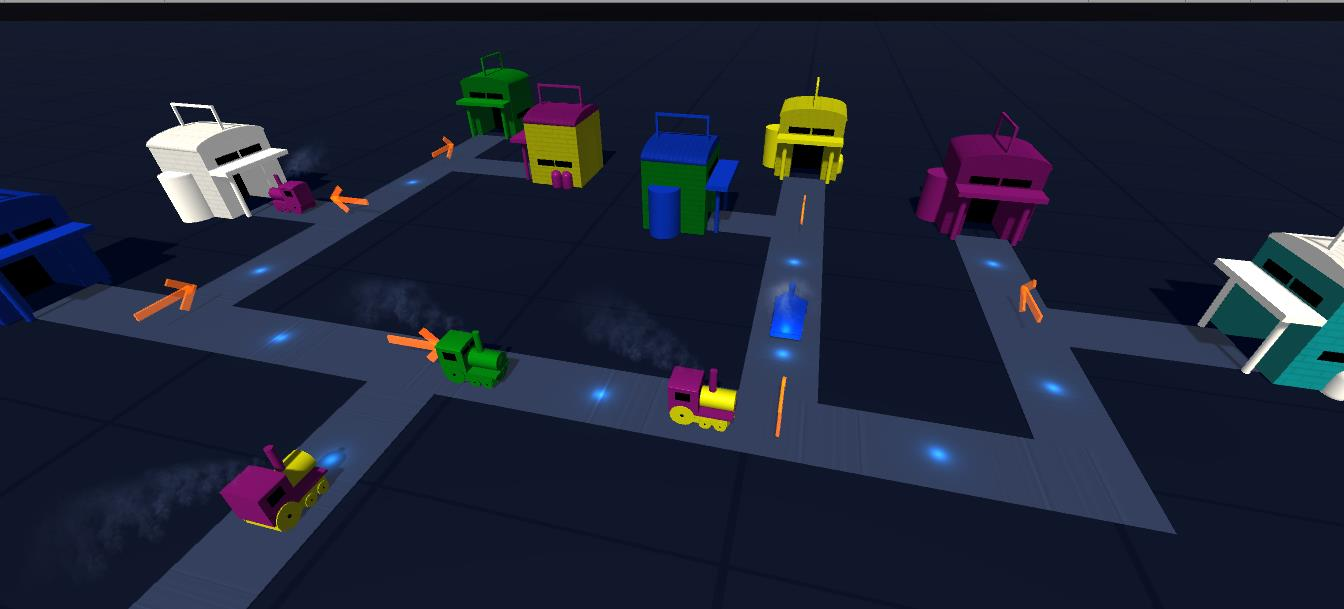
\includegraphics[width=0.325\textwidth]{images/parta.jpg}
\label{fig:parta}
}
\subfloat[Paquete de Velocidad]{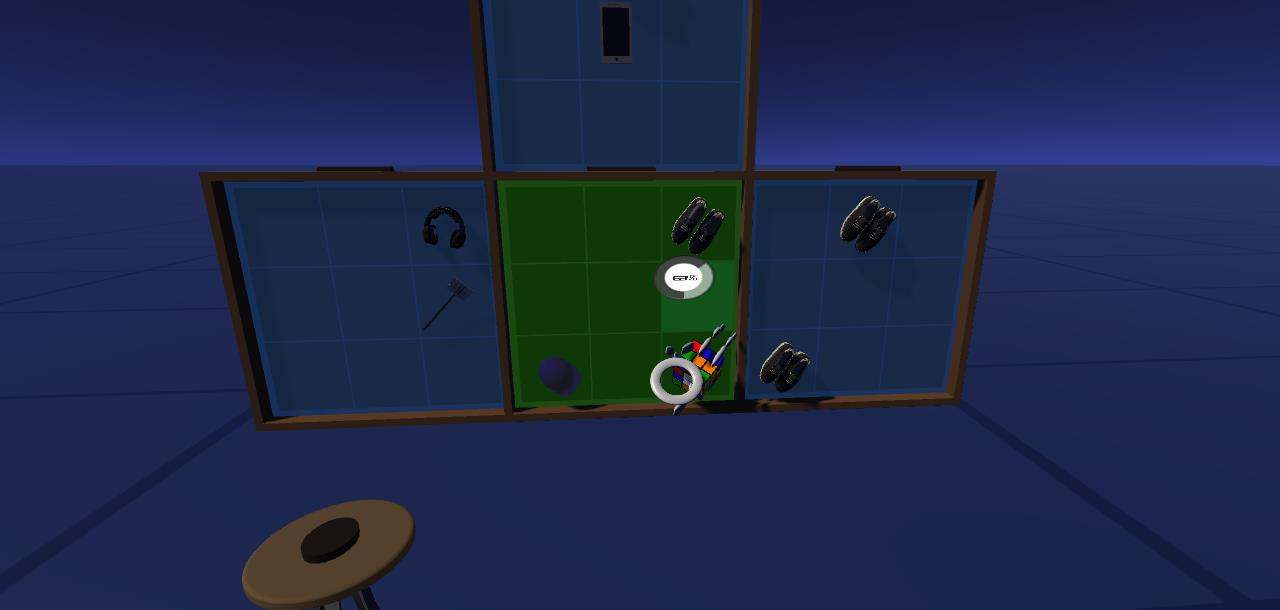
\includegraphics[width=0.325\textwidth]{images/partb.jpg}
\label{fig:partb}
}
\subfloat[Punto / Puntos]{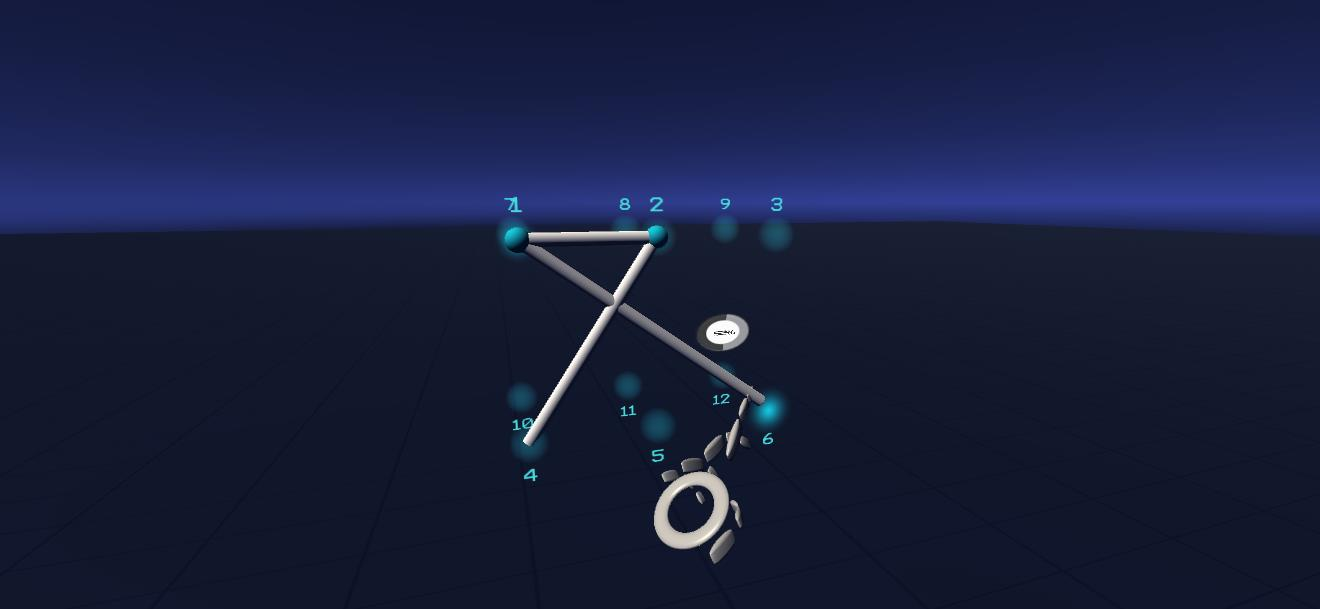
\includegraphics[width=0.325\textwidth]{images/partc.jpg} 
\label{fig:partc}
}
\end{tabular}
\caption{Muestra de un Instante en la Ejecución de los Juegos de Entrenamiento Planteados en Nuestra Propuesta}
\label{fig:scheme}
\end{figure*}


%%%%%%%%%%%%%%%%%%%%%%%%%%%%%%%%%%%%%%%%%%%%%%%%
\section{Soluci\'on Propuesta} \label{solucion}

La solución propuesta consta de una parte de hardware y software. Dado que se requiere que el usuario este inmerso dentro de un ambiente virtual, debe existir una interacción de este con el ambiente. El ambiente virtual se basa en juegos virtuales mostrados en la Figura \ref{fig:scheme}. La interacción la provee el dispositivo Leap Motion \cite{LEAP}, que es un pequeño dispositivo que emplea cámaras infrarrojas monocromáticas e infrarrojas de LED, permitiendo capturar el movimiento de las manos y dedos a una distancia de 1 m. Es un dispositivo similar a un ratón convencional de computador, pero sin contacto. Este dispositivo puede ser colocado en la parte frontal de un casco Oculus Rift \cite{OCULUS}, y así tener un ambiente de bajo costo para la creación de aplicaciones basadas en realidad virtual inmersiva.

En la Figura \ref {fig:scheme2} se muestra la configuración tanto del casco Oculus Rift, como del periférico Leap Motion dentro de la solución propuesta. Nótese que el caso no restringe la movilidad libre de la cabeza del usuario, y el Leap Motion no restringe el movimiento total de los brazos, manos y dedos del usuario.

\begin{figure}[htp]
\centering
\begin{tabular}{cc}
\subfloat[]{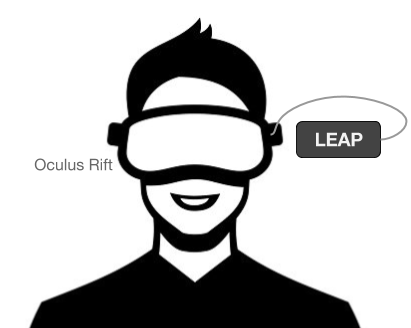
\includegraphics[width=0.5\columnwidth]{images/scheme.png}
\label{fig:fig1a}
}
\subfloat[]{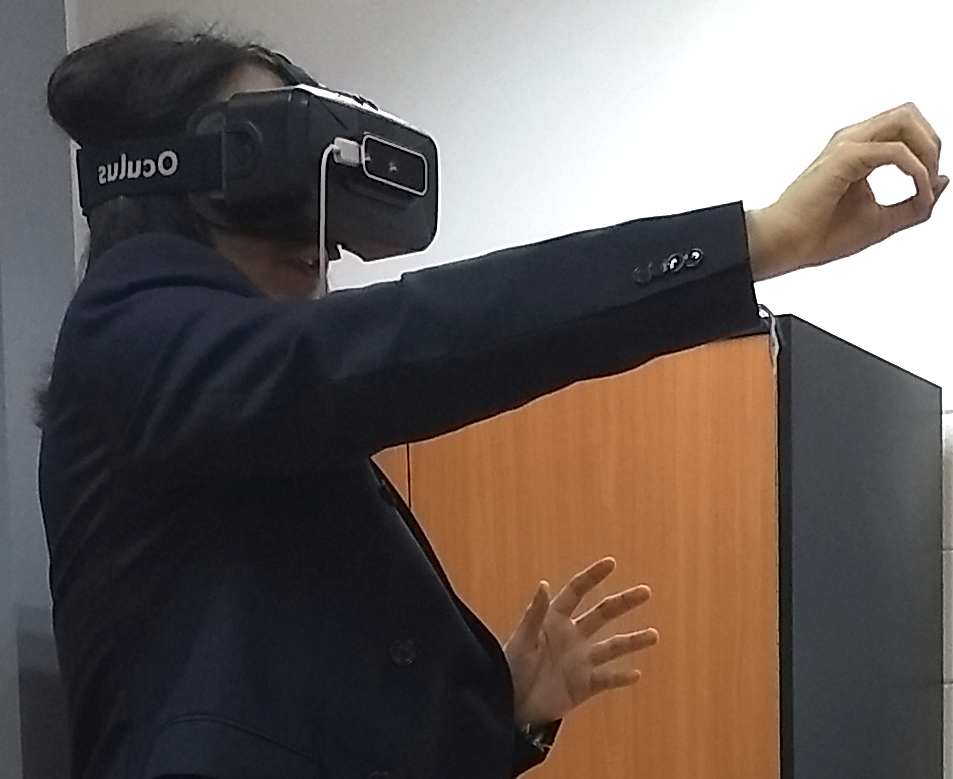
\includegraphics[width=0.45\columnwidth]{images/sam.png} \label{fig:fig1b}
}
\end{tabular}
\caption{Configuración de Nuestra Propuesta, Empleando (a) un Casco Oculus Rift y el Leap Motion, (b) así como su Disposición con el Usuario}
\label{fig:scheme2}
\end{figure}

Ambos dispositivos se comunican con un computador empleando puertos USB. Una vez configurado los dispositivos de hardware, se construyó una arquitectura de software que permite la captura de la interacción de los dispositivos con el usuario, así como el despliegue de diversas escenas 3D para su navegación. El usuario, podrá navegar dentro de dichas escenas controlando e interactuando con el movimiento de la cabeza y el movimiento de las manos. Cada escena e interacción están asociados a un método de entrenamiento. Por otro lado, se mantiene un control de acceso de usuarios, para que cada uno pueda manejar diferentes niveles de entrenamiento, así como obtener sus estadísticas.

De esta manera, se tiene una solución de hardware y software para el entrenamiento mental basado en un juego serio \cite{Michael:2005:SGG:1051239}, orientado a la inteligencia espacial bajo un ambiente de realidad virtual con el uso de dispositivos de bajo costo empleando movimientos gestuales. A continuación, se muestran los métodos de entrenamientos que son la base de nuestra solución. 
\bigskip

%%%%%%%%%%%%%%%%%%%%%%%%%%%%%%%%%%%%%%%%%%%%%%%%
%\subsection{M\'etodos de Entrenamiento}
\textit{A. M\'etodos de Entrenamiento}
\medskip

Los métodos de entrenamiento se componen principalmente por dos características fundamentales: la estimulación de ciertas áreas cognitivas y la interacción con el entorno. Dichas características fueron evaluadas en diferentes entrenamientos donde puedan adaptarse a un entorno de realidad virtual o aquellos que permitan mantener su función principal, pero cambiando el modo de interacción con el mismo. Por lo tanto, se seleccionaron y diseñaron tres entrenamientos:

%%%%%%%%%%%%%%%%%%%%%%%%%%%%%%%%%%%%%%%%%%%%%%%%
\subsubsection*{\textbf{Ruta de Enfoque}}

Consiste en la coincidencia de dos objetos del mismo color. Se genera una plataforma con una ruta preestablecida y una variedad de interruptores, dichos interruptores son controlados por el usuario e indican la dirección hacia donde debe de dirigirse un objeto movible (ver Figura \ref{fig:parta}). Los objetos estáticos serán colocados de manera aleatoria al final de cada ruta y a partir de ese momento comenzarán a circular los objetos movibles desde un único punto de salida donde se conecta con la ruta principal.

%%%%%%%%%%%%%%%%%%%%%%%%%%%%%%%%%%%%%%%%%%%%%%%%
\subsubsection*{\textbf{Paquete de Velocidad}}

Se basa en la colocación de un objeto dentro de un contenedor o paquete que contiene también otros objetos. Un contenedor o paquete está compuesto por varias partes o sub-paquetes, formando un plano en el espacio, cada sub-paquete contiene una variedad de objetos posicionados en un vector en particular (ver Figura \ref{fig:partb}). El objetivo principal del usuario consiste en situar el objeto faltante en alguna posición del paquete sin que se superponga con los demás objetos al momento que cierre. 

%%%%%%%%%%%%%%%%%%%%%%%%%%%%%%%%%%%%%%%%%%%%%%%%
\subsubsection*{\textbf{Punto / Puntos}}

Consiste en la unión de varios puntos con el fin de lograr una figura deseada, esta puede ser conocida o abstracta. Se le presenta al usuario una cierta cantidad de puntos simétricos y un modelo basado en dichos puntos, el usuario debe de lograr unir los puntos necesarios de manera linear para completar la figura buscada (ver Figura \ref{fig:partc}).

Las áreas cognitivas que presentan los entrenamientos previamente seleccionados consisten en: concentración, atención, agilidad o velocidad mental, modelación y memoria, como se muestra en la Figura \ref{fig:methods}. Basándose en dichas áreas y tomando en cuenta la adaptación de un entrenamiento a un entorno de realidad virtual, se diseñaron estimulaciones adicionales tales como la percepción, estimación y abstracción que podrán ser calculadas mediante un cierto tiempo de reacción que el usuario obtenga en los entrenamientos basándose en el comportamiento de cada uno.

\begin{figure}[htpb!]
 \centering 
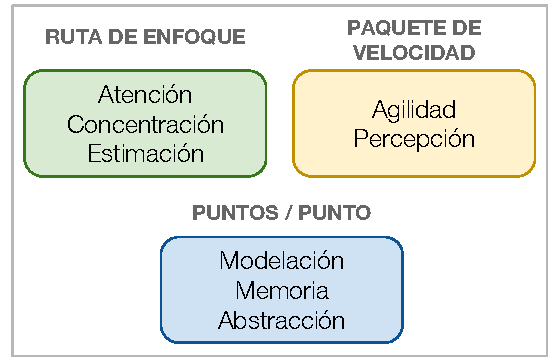
\includegraphics[width=1.0\columnwidth]{images/methods.pdf}
\caption{Áreas de Acción de cada Entrenamiento Propuesta}
\label{fig:methods}
\end{figure}

Los entrenamientos realizados son supervisados a través de un tiempo global para la realización del mismo. El tiempo varía según la dificultad y el tipo de entrenamiento definido. La definición operacional del grado de dificultad de la tarea es el tiempo de respuesta, ya que se supone que, a mayor grado de dificultad, mayor tiempo de procesamiento requerido para generar una respuesta apropiada.
%Las variables estadísticas utilizadas en la aplicación son basadas en el tiempo de respuesta para ejecutar una tarea, %ya que el cerebro reacciona a un estímulo cuando este se ve forzado a procesar una información y poder generar una respuesta apropiada.

Un ejemplo común para explicar este proceso, es el uso del tiempo para realizar un examen o evaluación a un estudiante. El cerebro del estudiante deberá procesar una información a partir de una pregunta, ya sea de desarrollo, y generar una respuesta en particular. No obstante, si la pregunta es de selección simple, el cerebro procesa la información utilizando un patrón para generar la respuesta que crea ser correcta. Para ambas preguntas, el cerebro se comporta y obtiene distintos tiempos de respuesta basándose en el tipo de pregunta que se le presente, suponiendo que el estudiante conoce efectivamente ambas respuestas. La velocidad de respuesta que el usuario obtenga en la aplicación permite a los algoritmos crear una estimación de resultados apropiados conforme a la complejidad del entrenamiento, generando valores aproximados de las estimulaciones realizadas.

Cabe destacar que, los resultados estimados por la aplicación no representan valores reales asociados a teorías sobre el proceso de estimulación que se adaptan al cerebro. Sin embargo, como se ha mencionado anteriormente, se sustentan bajo el principio básico del tiempo de respuesta que el cerebro presenta ante una tarea o actividad en particular.
\bigskip

%%%%%%%%%%%%%%%%%%%%%%%%%%%%%%%%%%%%%%%%%%%%%%%%
%\subsection{Base de Datos}
\textit{B. Base de Datos}
\medskip

La base de datos se inicia con la necesidad de almacenar la información correspondiente para los entrenamientos: modelos, estadísticas, actividades e interpretaciones gestuales. Esto se realiza en un modelo convencional de entidad-relación.  Los entrenamientos están compuestos por diferentes modelos que conforman una escena, algunos modelos pueden ser necesarios para la interpretación de gestos necesarios para la funcionalidad e interacción con la escena. La actividad corresponde al tipo de estimulación que posee cada entrenamiento y utilizada para el cálculo de las estadísticas del usuario. Por último, los criterios de evaluación y resultados que son manejados por las estadísticas y dependerán del desempeño del usuario obtenido en cada uno de los entrenamientos.

Los usuarios, y debido a que la aplicación no está diseñada para un entorno en la red, sólo tendrán que ingresar un nombre de usuario con el fin de poder guardar resultados asociados a dicho nombre, similar a los juegos tradicionales de Microsoft Windows como Solitario o 3D Pinball.
\bigskip

%%%%%%%%%%%%%%%%%%%%%%%%%%%%%%%%%%%%%%%%%%%%%%%%
%\subsection{Entidades 3D}
\textit{C. Entidades 3D}
\medskip

La solución fue desarrollada con el motor de videojuegos Unity3d \cite{UNITY} que permite la utilización de ciertos recursos que facilitan el manejo de datos. Los objetos programables o \textit{ScriptableObjects} son clases serializadas que permiten almacenar datos para compartir entre los componentes y evitar el acceso constante a base de datos. Los modelos utilizados en cada uno de los entrenamientos son almacenados en ScriptableObjects personalizados según el dominio de trabajo.

Los modelos fueron creados a partir de las funciones para posicionar, girar, expandir y agrupar objetos tridimensionales que ofrece Unity3d. Algunos objetos creados se muestran en la Figura \ref{fig:objects}. Algunos modelos fueron exportados directamente al entorno y por medio de archivos de tipo Object (.obj). Los modelos se clasifican en dos tipos: Estáticos y Dinámicos.

\begin{figure}[htpb!]
 \centering 
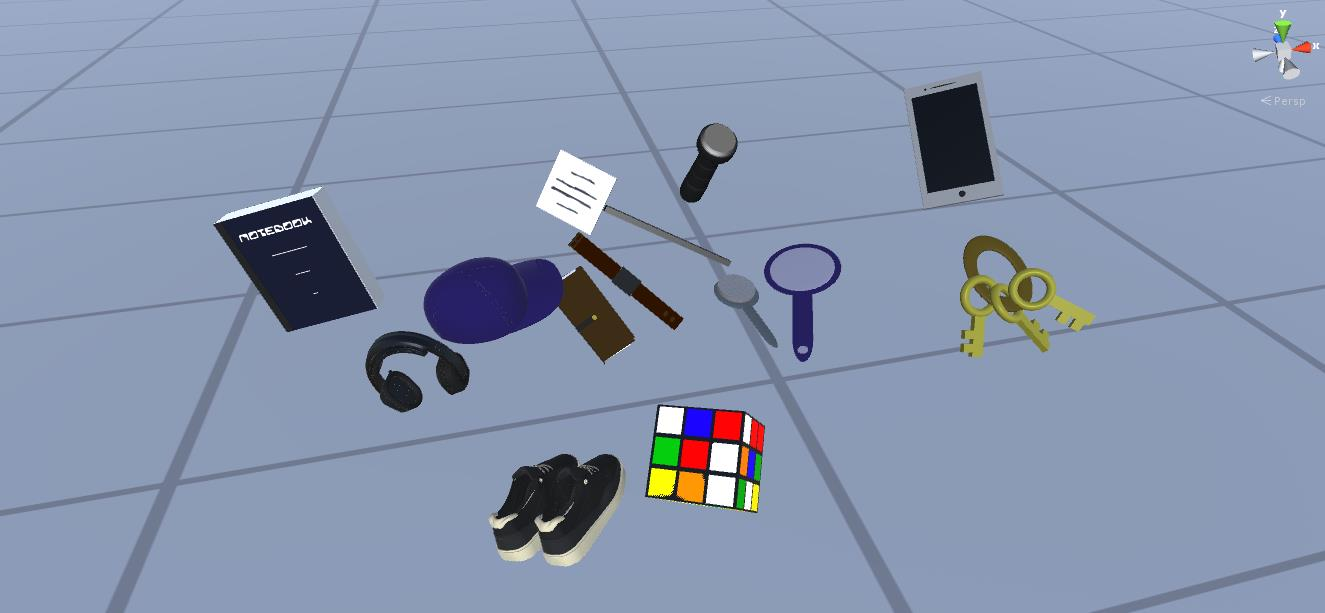
\includegraphics[width=1.0\columnwidth]{images/objects.jpg}
\caption{Modelos Creados del Tipo Estático o Dinámico}
\label{fig:objects}
\end{figure}

\begin{figure*}[htpb!]
\centering
\begin{tabular}{cc}
\subfloat[]{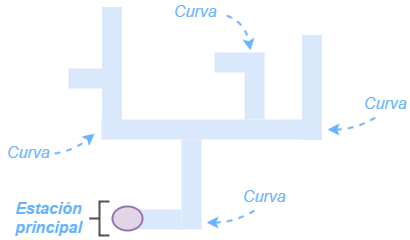
\includegraphics[width=0.32\textwidth]{images/rutasCurvas.png}
\label{fig:rutaa}
}
\subfloat[]{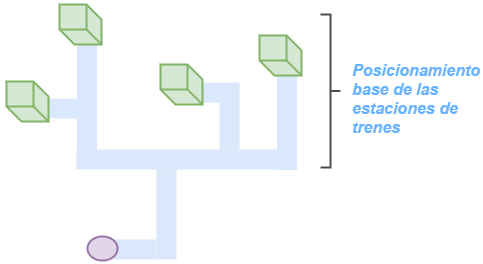
\includegraphics[width=0.37\textwidth]{images/estaciones.png}
\label{fig:rutab}
}
\subfloat[]{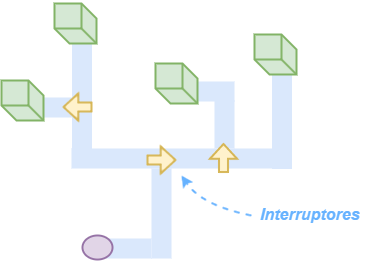
\includegraphics[width=0.28\textwidth]{images/final.png} 
\label{fig:rutac}
}
\end{tabular}
\caption{Esquema de las (a) Posiciones de las Rutas y Curvas, (b) las Inicialización de los Objetos, y (c) la Ubicación de los Interruptores}
\label{fig:rutas}
\end{figure*}

Los modelos estáticos pertenecen a la escena que representan y ambientan el entorno. Sin embargo, estos pueden ser creados en la escena sin componentes visuales manteniéndose como administradores de la escena. Los objetos dinámicos son aquellos que son inicializados a partir de un determinado momento, son almacenados en los \textit{ScriptableObjects} y se utilizan para la interacción con el usuario a través de scripts de comportamiento.

De esta forma, se asociaron scripts a cada modelo dinámico perteneciente a una escena. Cada script se basa en un componente de comportamiento que permiten manipular el objeto a través de código, ofreciendo un intercambio de información entre los modelos a través de un determinado evento. Cada escena contiene un script administrador asignado a un único modelo. Esto permite manejar y controlar las responsabilidades funcionales entre el comportamiento de cada uno de los modelos principales de la escena y la interacción con el usuario.
\bigskip

%%%%%%%%%%%%%%%%%%%%%%%%%%%%%%%%%%%%%%%%%%%%%%%%
%\subsection{Leap Motion}
\textit{D. Leap Motion}
\medskip

A lo largo del desarrollo de los modelos generales, se mencionará la utilización de un controlador LeapHand para la ejecutar una cierta acción o tarea. Un controlador LeapHand es el medio por el cual el usuario interactúa con la aplicación que refleja la posición de las manos en el mundo virtual. El controlador es diseñado conforme a las exigencias que requiere un dominio en particular, es decir, está compuesto por distintos elementos y scripts de comportamiento para la captura de información. Se emplearon cuatro gestos principales a partir de los controladores asociados a la API del LeapHand descritas a continuación:

\begin{itemize}
\item \textbf{Toque}: Consiste en el uso del dedo índice del controlador para activar un objeto por medio de una colisión. Las colisiones son reconocidas por el objeto a través de etiquetas asignadas al componente del dedo índice. Cuando el objeto colisionado detecta un toque, se habilitan las variables físicas del objeto, permitiendo que este reaccione a la fuerza recibida por la colisión y pueda ejecutar una acción.
\item \textbf{Doble Toque}: Presenta un comportamiento similar al gesto de Toque con la diferencia de que la etiqueta de colisión es asignada también al dedo medio del controlador. Es utilizado para acciones donde se requiera de mayor rapidez para realizar una acción. 
\item \textbf{Agarre}: Consiste en posicionar el controlador en una forma de agarre, es decir, la distancia entre la posición de punta de los dedos con respecto al punto centro de la palma sea menor que un umbral. Se utilizan vectores unitarios normalizados para obtener una distancia en el espacio. Para que ocurra el Agarre, el objeto candidato a ser agarrado debe estar identificado con una etiqueta que indique si es posible ser sostenido por el controlador.
\item \textbf{Palma arriba}: Se basa en girar la palma del controlador hacia arriba, es decir, consiste en conocer el valor de la posición en un eje $Y$ del vector director de la palma. Cuando este valor es igual a 0.5 unidades aproximadamente, se obtiene una palma girada unos $90^{\circ}$. Las acciones se activan cuando la palma haya girado al menos hasta un valor aproximado de 0.6 unidades.
 \end{itemize}

%%%%%%%%%%%%%%%%%%%%%%%%%%%%%%%%%%%%%%%%%%%%%%%%
%%%%%%%%%%%%%%%%%%%%%%%%%%%%%%%%%%%%%%%%%%%%%%%%

\section{Entrenamientos} \label{training}

Como se mencionó anteriormente, se han desarrollado tres métodos de entrenamiento cognitivos bajo un ambiente de realidad virtual: Ruta de Enfoque, Paquete de Velocidad y Puntos/Punto. Cada uno de estos, posee distintos niveles de dificultad: básico, medio y avanzado. A continuación, se mostrará más detalle de cada uno de estos.
\bigskip

%%%%%%%%%%%%%%%%%%%%%%%%%%%%%%%%%%%%%%%%%%%%%%%%
%\subsection{Rutas de Enfoque}
\textit{A. Rutas de Enfoque}
\medskip

Para el diseño de este entrenamiento, se distribuyeron un conjunto de objetos 3D estáticos y dinámicos. Existirá un tren como objeto principal (dinámico) que debe pasar por diversas estaciones (estático). Así, cada tren iniciará en un único punto de salida con un color en particular, definido de forma pseudoaleatoria, a partir de este momento iniciará su recorrido por medio de las rutas hacia una estación, donde esta última iniciará a su vez con un color definido aleatoriamente. El usuario se encargará de interactuar con los botones asociados a los interruptores para realizar los cambios de dirección respectivos y guiar a cada uno de los trenes que circulan en la plataforma a la estación del color adecuado. 

De acuerdo a la dificultad, ciertos objetos son instanciados y colocados dentro de la escena 3D.  El posicionamiento final de las rutas y curvas se puede observar en la Figura \ref{fig:rutas}a. Para realizar la creación de rutas y curvas, se cargan los distintos modelos y posicionarlos a partir de la estación principal, dicha estación indica el punto inicial de los trenes que circularán. Cuando la inicialización de las rutas culmina, se procede con el indicador de curvas para una ruta en específico, es decir, se colocan las curvas según el modelo de ruta.

% \begin{figure}[htpb!]
%  \centering 
% 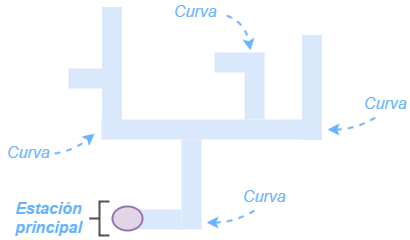
\includegraphics[width=1.0\columnwidth]{images/rutasCurvas.png}
% \caption{Posiciones de las rutas y curvas base en Rutas de Enfoque.}
% \label{fig:rutas}
% \end{figure}

Las estaciones se inicializan a partir del final de una ruta indicada, como se puede observar en la Figura \ref{fig:rutas}b, se selecciona un color al azar y se asigna una posición en la escena (que se denomina plataforma). Una vez inicializada, se le asigna a cada modelo de estación su objeto lógico que permitirá generar las validaciones necesarias para la llegada de cada tren.

% \begin{figure}[htpb!]
%  \centering 
% 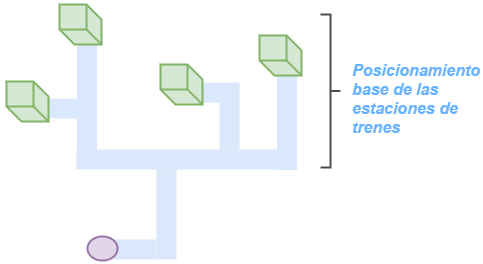
\includegraphics[width=1.0\columnwidth]{images/estaciones.png}
% \caption{Posicionamiento base de las estaciones en Rutas de Enfoque.}
% \label{fig:estaciones}
% \end{figure}

Para que el tren cumpla el objetivo de llegar a su destino (bases), existen una serie de interruptores que permiten cambiar la dirección del tren. Las posiciones de los interruptores se inicializan de forma predeterminada basada en la dificultad seleccionada, para cada uno existe una dirección pseudoaleatoria a la propiedad del modelo. Seguidamente se inicializa y se asocia un botón encargado del cambio de dirección. El resultado final de este proceso de inicialización se muestra en la Figura \ref{fig:rutas}c.

% \begin{figure}[htpb!]
%  \centering 
% 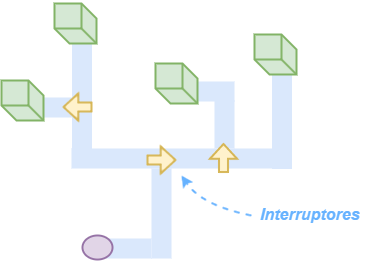
\includegraphics[width=0.9\columnwidth]{images/final.png}
% \caption{.}
% \label{fig:final}
% \end{figure}

Por otro lado, el movimiento del tren consiste en el resultado de un vector de dirección por un escalar de velocidad $v$ y un tiempo $t$, obteniendo como resultado el vector de posición que es utilizado por el controlador para trasladarse a sí mismo a través de las rutas. El valor de $V$ permanecerá constante durante todo el recorrido del tren y, $t$ es obtenido por medio de los cuadros por segundo del controlador. Esta ecuación se esquematiza en la Figura \ref{fig:tren}. La rotación del tren puede ejecutarse debido a una curva o mediante la dirección de un interruptor, siendo necesario que el tren reconozca cada uno de los casos.

\begin{figure}[htpb!]
 \centering 
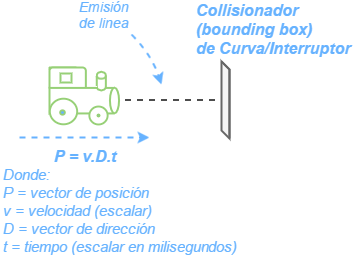
\includegraphics[width=0.7\columnwidth]{images/tren.png}
\caption{Movimiento y Emisión de Línea de un Tren}
\label{fig:tren}
\end{figure}

Para la rotación por curva se asignó una etiqueta de identificación a los modelos de curva que permiten al tren reconocer la colisión de un objeto en particular, una vez detectada la colisión, el controlador del tren obtiene la información de la curva indicando hacia donde debe de girar. La rotación por interruptor es muy similar la rotación por curva, con la diferencia que el controlador del tren, una vez detectada la colisión con un interruptor, activa parámetros que previenen que el tren gire nuevamente si este aún sigue colisionando con el mismo interruptor.

La llegada de cada tren, se valida a través de la presencia de una colisión continua con una estación. De esta manera, la colisión del tren persiste por un pequeño lapso del tiempo con el propósito de generar una sensación de entrada a dicha estación. Una vez transcurrido el tiempo se realiza la coincidencia de color y se almacena el resultado, en este punto el ciclo de vida del modelo de tren culmina y es eliminado de la plataforma.

%%%%%%%%%%%%%%%%%%%%%%%%%%%%%%%%%%%%%%%%%%%%%%%%
\subsubsection*{Interacci\'on}

La interacción del usuario con el juego se basa en un panel que contiene cada uno de los botones asociados a un interruptor, representando todas las rutas y los interruptores en forma de miniatura. La configuración de sensibilidad del botón depende de la distancia con respecto a la posición del usuario, el tamaño y el peso físico del modelo.

Los indicadores de los botones consisten en una animación que permite identificar visualmente a cuál interruptor pertenece un botón, con el propósito de mejorar la experiencia de usuario y lograr la familiarización con el entorno al momento de ingresar al entrenamiento. La animación se basa en una flecha flotante sobre el interruptor y un efecto de luz sobre el botón asociado. 

Empleando el dedo índice, se lanza un rayo que permite realizar la intersección entre una línea y el objeto que componen a los botones. Cuando una línea colisiona con un botón, se activan los indicadores del interruptor siempre y cuando la colisión persista con el mismo botón, de otra manera, los botones vuelven a su estado original (i.e. no seleccionados).


%%%%%%%%%%%%%%%%%%%%%%%%%%%%%%%%%%%%%%%%%%%%%%%%
\subsubsection*{Puntuación y Estadísticas}

La solución propuesta, tiene entre sus funciones la administración del tiempo de un entrenamiento, contando el tiempo de inicio y el tiempo total mostrando un panel visible para el usuario. El tiempo de inicio consiste en cinco segundos de preparación antes de la inicialización de trenes. De igual manera, se indica al momento de culminar el tiempo general, que consiste en tres minutos a partir del primer tren inicializado. El entrenamiento no culmina hasta que todos los trenes hayan llegado a su destino.

La puntuación se basa en un contador total de trenes y los aciertos que haya realizado el usuario. El contador se va incrementado a medida que vayan llegando trenes a una estación, donde a partir de cada llegada de los trenes se evalúan los datos obtenidos en todo su recorrido. Los datos para la evaluación estadística consisten en una variedad de criterios aplicados sobre el tren en un intervalo de tiempo de dos segundos antes de la colisión con un interruptor:
\begin{enumerate}
\item El tren llega a su respectiva estación y el usuario no haya realizado cambios de dirección del interruptor dentro del intervalo.
\item El tren llega a su respectiva estación y el usuario haya realizado uno o varios cambios de dirección del interruptor dentro del intervalo.
\item El tren no llega a su respectiva estación y el usuario no haya realizado cambios de dirección del interruptor dentro del intervalo.
\item El tren no llega a su respectiva estación y el usuario haya realizado uno o varios cambios de dirección del interruptor dentro del intervalo.
\end{enumerate}

Estos datos son recopilados para su análisis y almacenamiento, y una vez culminado el entrenamiento se muestra al usuario los resultados finales del entrenamiento: nivel de atención, concentración y la puntuación general.
\bigskip

%%%%%%%%%%%%%%%%%%%%%%%%%%%%%%%%%%%%%%%%%%%%%%%%
%\subsection{Paquete de Velocidad}
\textit{B. Paquete de Velocidad}
\medskip

\begin{figure*}[htpb!]
\centering
\begin{tabular}{cc}
\subfloat[Algunos Tipos de Sub-paquetes en Paquete de Velocidad]{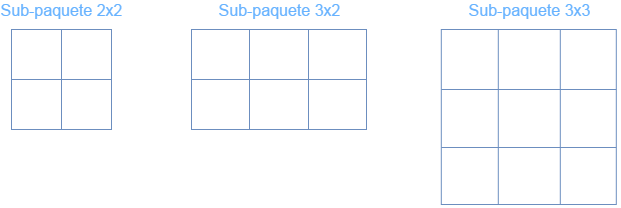
\includegraphics[width=0.42\textwidth]{images/paquete.png}
\label{fig:paquetea}
}
\subfloat[Orientaciones de los Sub-paquetes en Paquete de Velocidad]{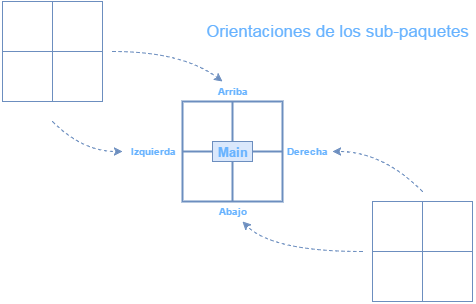
\includegraphics[width=0.42\textwidth]{images/subpaquete.png}
\label{fig:subpaquete}
}
\end{tabular}
\caption{Organización y Estructuras de los Paquetes}
\label{fig:paquete}
\end{figure*}

En el diseño del entrenamiento Paquete de Velocidad, se plantea la selección de un tipo de paquete. Donde, un paquete es manipulado por una entidad encargada de efectuar la configuración de sus respectivas partes (o sub-paquetes), y proceder con distintos algoritmos de posicionamiento para los objetos estáticos en un espacio en particular. Una vez finalizado dicho proceso, se habilita un objeto manejable que consiste principalmente en el medio por el cual el usuario podrá interactuar con el escenario actual. 

Un paquete se define como un modelo lógico compuesto por dos o más sub-paquetes físicos representados como una matriz plana en el espacio con un tamaño mínimo de $2 \times 2$. Para que exista un paquete es necesario la existencia de al menos dos sub-paquetes con una orientación en particular, en la Figura \ref{fig:paquetea} se muestran algunas configuraciones ejemplo de paquetes utilizados en el entrenamiento.


% \begin{figure}[htpb!]
%  \centering 
% 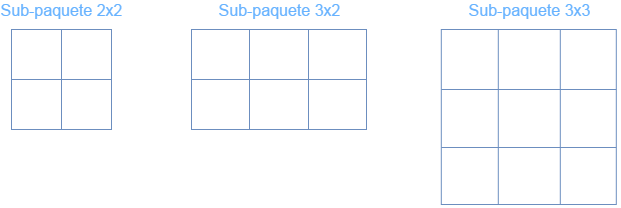
\includegraphics[width=1.0\columnwidth]{images/paquete.png}
% \caption{Algunos tipos de sub-paquetes en Paquete de Velocidad.}
% \label{fig:paquete}
% \end{figure}

La configuración consiste en determinar el tipo o modelo lógico del paquete, asignar un sub-paquete principal y utilizar la orientación de éste modelo para realizar la inicialización, teniendo como resultado un paquete donde el usuario podrá colocar el objeto faltante en un algún espacio disponible. Se realizan las validaciones necesarias y se repite el proceso hasta la culminación del tiempo disponible.

La configuración de un paquete consiste en dos pasos: 1) elegir un sub-paquete y, 2) otorgar el rol de principal. El rol de principal es fundamental para el proceso de distribución e inicialización de objetos, y seguidamente la lectura de orientación del tipo de paquete previamente seleccionado. En la Figura \ref{fig:subpaquete} se puede observar las cuatro orientaciones de los sub-paquetes y dependiendo de la orientación que contenga el sub-paquete, el algoritmo de distribución e inicialización de objetos varía.


% \begin{figure}[htpb!]
%  \centering 
% 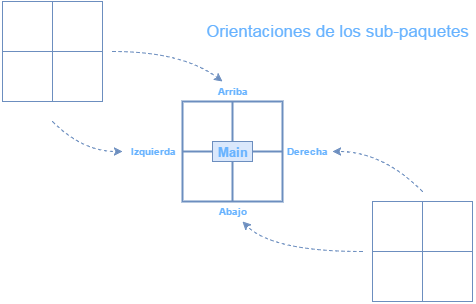
\includegraphics[width=1.0\columnwidth]{images/subpaquete.png}
% \caption{Orientaciones de los sub-paquetes en Paquete de Velocidad.}
% \label{fig:subpaquete}
% \end{figure}

Por ejemplo, dado un paquete compuesto de tres sub-paquetes, si el sub-paquete con el rol principal tiene una orientación a la izquierda, se selecciona uno de los dos sub-paquetes restantes, donde será configurado e inicializado a la izquierda del principal, y para el último sub-paquete, dependiendo de la clase estrategia seleccionada al principio del proceso de creación. Entonces, dicho paquete será configurado e inicializado según la orientación del segundo sub-paquete.
%(ver Fig \ref{fig:compaquete}).

% \begin{figure}[htpb!]
%  \centering 
% 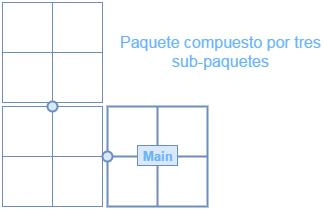
\includegraphics[width=0.75\columnwidth]{images/compaquete.png}
% \caption{Paquete compuesto por tres sub-paquete en Paquete de Velocidad.}
% \label{fig:compaquete}
% \end{figure}

La distribución e inicialización de objetos se basa en la creación de una lista lógica de objetos que son asignados al sub-paquete principal, y a partir de esta se selecciona una cierta cantidad de objetos para después ser reflejados en los sub-paquetes restantes. Primeramente, el sub-paquete principal inicializa una variedad de objetos y los descarta de la lista, deshabilitando los espacios donde estos son inicializados con el fin de evitar superponer la posición con otro objeto. Luego, es enviada la lista con los objetos faltantes al paso de distribución. El algoritmo de distribución consiste básicamente en buscar una posición espejo a partir del sub-paquete precedente y reflejarlos al sub-paquete seleccionado, en caso de existir algún otro sub-paquete, el proceso se repite. 

En la Figura \ref{fig:ecespejo} se muestra la ecuación empleada para reflejar un objeto a un sub-paquete adyacente. A nivel de comunicación entre los módulos internos de la solución, se requiere enviar como parámetros la orientación entre los dos sub-paquetes, el tamaño máximo del vector $XY$ y la posición $(x,y)$ actual del objeto sobre la matriz. Para una orientación Derecha-Izquierda se utiliza la variable $X$, mientras que para una orientación Arriba-Abajo se utiliza la ecuación con variable $Y$. Con la nueva posición espejo, el sub-paquete actual almacenará el objeto en su estructura de datos, y este procederá con su respectiva inicialización.


\begin{figure}[htpb!]
 \centering 
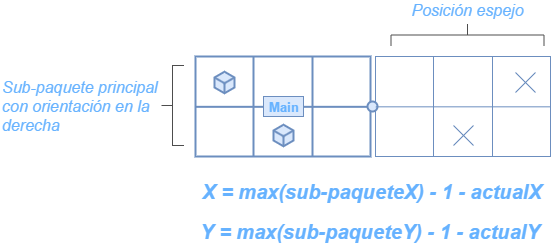
\includegraphics[width=1.0\columnwidth]{images/ecespejo.png}
\caption{Ecuación para Obtener la Posición Espejo en Paquete de Velocidad}
\label{fig:ecespejo}
\end{figure}

%%%%%%%%%%%%%%%%%%%%%%%%%%%%%%%%%%%%%%%%%%%%%%%%
\subsubsection*{Interacci\'on}

En la interacción en este entrenamiento, además de las intersecciones rayo-botones, se requiere que el usuario pueda agarrar, arrastrar y soltar (i.e. \textit{drag \& drop}). Por ello, %como se observa en la Fig \ref{fig:restriccion}, 
se deben considerar que un objeto tiene ciertas propiedades físicas básicas dentro de un ambiente virtual como el desplazamiento y la gravedad. A este tipo de objetos, dentro de la solución se les identifica como objetos manejables.

% \begin{figure}[htpb!]
%  \centering 
% 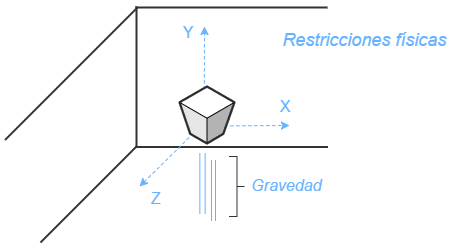
\includegraphics[width=1.0\columnwidth]{images/restriccion.png}
% \caption{Restricciones físicas de un objeto.}
% \label{fig:restriccion}
% \end{figure}

La manipulación de las restricciones consiste en anular cualquier tipo de fuerza física que pueda estar presente al momento de retener el objeto, evitando comportamientos o efectos de rebote. Es importante destacar, que el controlador LeapHand ocasiona una serie de diversas colisiones contra el objeto en distintos ángulos, es decir, se generan distintas fuerzas en varias direcciones, produciendo el efecto de rebote en el controlador LeapHand que se busca eliminar.

El controlador LeapHand emite una línea a través de la palma, como se puede observar en la Figura \ref{fig:colision}. Si esta línea atraviesa la caja delimitadora (i.e. \textit{bounding box}) que rodea al objeto, se procede con la anulación de las restricciones físicas del objeto. Cuando no existen restricciones en el objeto, el usuario puede realizar un gesto de agarre con el cual logrará sujetar el objeto y arrastrarlo a un punto en particular, el cálculo del gestor de agarre se basa en un algoritmo de distancia entre los dedos índice y medio contra el pulgar, obteniendo una posición particular utilizada como punto de agarre entre el objeto y el controlador LeapHand.

\begin{figure}[htpb!]
 \centering 
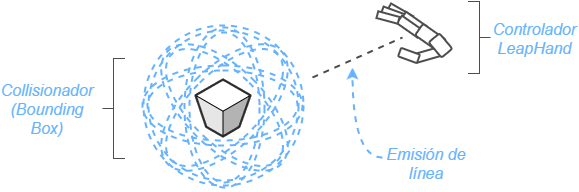
\includegraphics[width=1.0\columnwidth]{images/colision.png}
\caption{Área de Colisión y Línea de Emisión}
\label{fig:colision}
\end{figure}

Cuando un objeto manejable es colocado sobre algún espacio disponible, el controlador busca al sub-paquete más externo que posteriormente será eliminado. Así, la información se transfiere al sub-paquete anterior y se activa un método de animación que consiste en unir este último con el anterior, generando visualmente una transición en los objetos de ambos sub-paquetes. Este proceso se repite hasta llegar al sub-paquete principal, el cual adquiere, a este punto, todos los objetos inicializados con la excepción de que también estará el objeto colocado por el usuario. De esta forma, se podrá observar si este se ha sobrepuesto sobre alguno de los objetos que pertenecen al paquete.

Por otra parte, se debe realizar una comprobación de la superposición de los objetos. Esta consiste en obtener la posición del espacio donde fue colocado el objeto y recorrer la lista de objetos existentes. Si la posición obtenida no existe en la lista, entonces es considerado un acierto y se obtiene la puntuación correspondiente al tipo de paquete, en caso contrario se considera un fallo. Cuando se coloca el objeto manejable, se inicializa un verificador con el propósito de generar un efecto amigable con el entorno indicándole al usuario si ha logrado un acierto o ha realizado un fallo en la resolución del problema, y a partir de este momento se repite todo el proceso de creación e inicialización de paquetes.

%%%%%%%%%%%%%%%%%%%%%%%%%%%%%%%%%%%%%%%%%%%%%%%%
\subsubsection*{Puntuación y Estadísticas}

El tiempo total del entrenamiento es de dos minutos exactos. Tal como el entrenamiento de Paquete de Velocidad, existe un tiempo de cinco segundos de preparación antes de la inicialización del primer paquete. La puntuación consiste en un contador que se incrementa de acuerdo al paquete que se logre resolver, un contador para la cantidad de paquetes inicializados y un último contador correspondiente a los aciertos realizados. Como el entrenamiento tiene como finalidad estimular la agilidad mental, es indispensable llevar la suma del puntaje que se va obteniendo a medida que se resuelve cada paquete.
Los datos para la evaluación estadística se basan en tres variables por cada tarea, estos se van recolectando a partir de la inicialización de un paquete:

\begin{itemize}
\item Tiempo de colocación: Calcula el tiempo de percepción y reacción del usuario inmediatamente después que es mostrado un paquete.
\item Número de objetos: La cantidad de objetos inicializados y su respectiva distribución varía en la dificultad para la resolución de cada paquete.
\item Tipo de paquete: Similar a la cantidad de objetos, el tipo de paquete (dimensión y número de sub-paquetes que lo conforman) genera distintas dificultades para la resolución, existiendo una puntuación diferente para cada uno de los tipos.
\end{itemize}

En este entrenamiento, se muestra al usuario su desempeño como agilidad, percepción y la puntuación general.
\bigskip

%%%%%%%%%%%%%%%%%%%%%%%%%%%%%%%%%%%%%%%%%%%%%%%%
%\subsection{Punto / Puntos}
\textit{C. Punto / Puntos}
\medskip

En este entrenamiento, se deben construir líneas uniendo un conjunto de puntos siguiendo un patrón. Como estructura de datos, un conjunto de puntos seleccionados por el usuario se denomina modelo. Cuando un modelo es construido y asignado, el usuario interactuará con los puntos en la escena y podrá juntar o unir cada uno para formar líneas entre ellos. El usuario interactúa con los puntos de manera continua, es decir, si interactúa con un punto, este deberá trazar la línea hacia algún otro punto, sin embargo, tendrá la oportunidad de cancelar la selección del punto actual.

La construcción de un modelo consiste en crear una lista de puntos asociados entre sí que admite la repetición un punto más de una vez. Cada modelo seleccionado para el proceso de construcción permite hasta un cierto límite de asociaciones, el límite aumenta o disminuye según la dificultad seleccionada. En la Figura \ref{fig:conpuntos} se observa un ejemplo de la cantidad de puntos que pueden ser asociados a un modelo en particular.

\begin{figure}[htpb!]
 \centering 
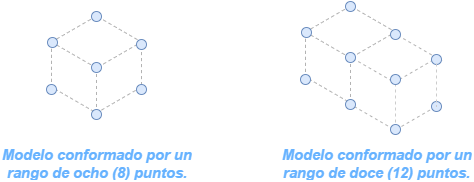
\includegraphics[width=1.0\columnwidth]{images/conpuntos.png}
\caption{Cantidad de Puntos Asociados a un Modelo en Punto / Puntos}
\label{fig:conpuntos}
\end{figure}

La construcción y creación de un modelo se hace de acuerdo a la selección del usuario en una dificultad previamente seleccionada. Cada punto está numerado según el orden de creación, así, un modelo se conforma por la selección de un conjunto de puntos distribuidos simétricamente. Cada modelo contiene una lista de puntos asociados que componen una figura en el espacio.

Los puntos contienen una lista de puntos asociados, llamados puntos vecinos. Esta lista permite reconocer todos los puntos vecinos que contiene el modelo a partir de uno en particular. Cuando se define la cantidad de puntos que conforman a un modelo, se procede con la inicialización de las líneas a partir de un punto inicial y un punto final. La inicialización de líneas permite generar el modelo visual utilizado por el usuario como ejemplo y referencia del objetivo del entrenamiento.

El proceso de inicialización de líneas consiste en un bucle donde se recorre la lista de puntos correspondientes al modelo. A partir de un punto base de la lista, se inicializan las líneas correspondientes al par seleccionado. Una vez construido el modelo, se crea otra secuencia de puntos con el mismo orden de creación, enumeración y distribuidos para ser inicializados en la escena, asignándoles los valores de los puntos que posee el modelo creado. Este proceso es muy similar a la búsqueda por amplitud en un grafo (BFS – \textit{Breadth First Search}).

La asignación de valores genera un apuntador lógico desde el punto en la escena con el punto que conforma al modelo, permitiendo manipular los datos y valores del punto mientras este permanezca en la escena del entrenamiento. La Figura \ref{fig:secupuntos} muestra una secuencia de modelación con tres puntos seleccionados.

\begin{figure}[htpb!]
 \centering 
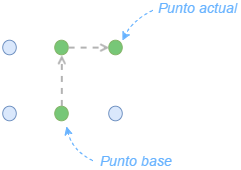
\includegraphics[width=0.7\columnwidth]{images/secupuntos.png}
\caption{Cantidad de Puntos Asociados a un Modelo en Punto / Puntos}
\label{fig:secupuntos}
\end{figure}


%%%%%%%%%%%%%%%%%%%%%%%%%%%%%%%%%%%%%%%%%%%%%%%%
\subsubsection*{Interacci\'on}

La interacción en este entrenamiento se enfoca en dos comportamientos principales: colisión y gestor de rotación. El comportamiento para la colisión consiste en asignar componentes físicos al dedo índice para el reconocimiento de objetos específicos. Existen dos tipos de componentes físicos con distintas responsabilidades según la orientación de la mano. Para la mano izquierda, el componente asignado al dedo índice reaccionará a la colisión de un punto inicializado en la escena, permitiendo la creación de líneas para la construcción del modelo solicitado, a partir de esta interacción, el usuario puede modelar una figura. Para la mano derecha, el componente físico reaccionará cuando colisiona con un punto en la escena cuando el punto ya ha colisionado con el componente de la izquierda. Esta última reacción es para anular el punto seleccionado por el usuario, permitiendo regresar a un paso anterior en la secuencia de modelación, o cancelar la secuencia. 

Desde el punto de vista del usuario, las líneas representan el medio por el cual se podrá visualizar los modelos a construir. En cada cuadro de despliegue, una línea debe ser transformada adecuadamente (e.g. escalamiento, rotación) de acuerdo a la posición del controlador LeapHand. Del mismo modo, cuando existe una intersección entre el componente del controlador con un punto de la escena, se activan dichas transformaciones. De este modo, la configuración del vector de tamaño, o escalamiento, consiste en modificar constantemente su factor de escala mientras no esté contenido dentro del área de colisión del controlador LeapHand (ver Figura \ref{fig:comtam}).

\begin{figure}[htpb!]
 \centering 
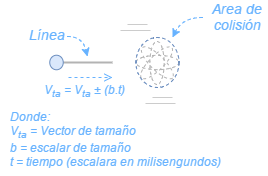
\includegraphics[width=0.80\columnwidth]{images/comtam.png}
\caption{Comportamiento del Vector de Tama\~no en Punto / Puntos}
\label{fig:comtam}
\end{figure}

El vector de tamaño se va modificando constantemente mediante un tiempo $t$ y un valor escalar de tamaño $b$. El funcionamiento tiene como propósito final, de manera visual, dejar la línea adherida al dedo índice del controlador LeapHand. Sin embargo, sin la configuración necesaria para el vector de rotación, este funcionamiento sólo aumentará o disminuirá de tamaño y no apuntará a la posición actual del controlador. La configuración del vector consiste en actualizar el vector director de una línea con respecto al dedo índice del controlador (i.e. vector normalizado).

Un modelo se compone por puntos, los cuales deben interactuar entre las intersecciones entre el componente LeapHand y la escena 3D donde residen los puntos. Cuando el evento de colisión se activa por medio del controlador LeapHand, existen tres comportamientos diferentes:

\begin{itemize}
\item Primera colisión: Se ejecuta cuando no ha iniciado la secuencia de puntos por parte del usuario, es decir, el primer punto seleccionado a partir de la construcción del modelo a completar.
\item Colisión a partir de una secuencia: Se ejecuta cuando existe una secuencia, el usuario ha desplazado la línea a un punto en particular y este desea colocarlo. Si el usuario mantiene la colisión con el punto donde desea colocar la línea, se procede con incorporar un nuevo elemento a la secuencia principal y se realiza la validación de la unión del par de puntos.
\item Colisión con el dedo índice del controlador derecho: Se ejecuta si existe una secuencia creada. Este comportamiento es utilizado para retornar a la secuencia anterior.
\end{itemize}

De este modo, la validación de un punto consiste en revisar y recorrer la lista del modelo base, y comparar el par de puntos unidos. Si un punto $A$ contiene como vecino a un punto $B$, entonces la unión es correcta, en caso contrario se considera un error. Cuando el usuario decide culminar el modelo construido, se revisa la cantidad de errores obtenidos, en caso de no haber ningún error, se considera un acierto.

%%%%%%%%%%%%%%%%%%%%%%%%%%%%%%%%%%%%%%%%%%%%%%%%
\subsubsection*{Puntuación y Estadísticas}

El tiempo para este entrenamiento consiste en cinco minutos, dado que requiere una mayor interacción con el entorno. El puntaje consiste en registrar la cantidad de aciertos logrados junto con la cantidad total de modelos generados. La cantidad de revelaciones consiste en el llevar el control de todas las revelaciones que realice el usuario para completar un modelo. El valor obtenido de revelaciones es utilizado para realizar el cálculo de las estimulaciones del entrenamiento.

Para la evaluación, se considera el tiempo de realización del modelo y los aciertos. Sin embargo, estos se sustentan por la cantidad de revelaciones realizadas utilizando el valor obtenido. Un valor de revelaciones se considera negativo a partir de la segunda revelación, ya que el entrenamiento tiene como finalidad fomentar la capacidad de abstracción y memoria del usuario


%%%%%%%%%%%%%%%%%%%%%%%%%%%%%%%%%%%%%%%%%%%%%%%%
\section{Experimentación} \label{tests}

La propuesta se compone principalmente en una aplicación basada en un entorno de realidad virtual, por lo que una medición del rendimiento es indispensable. Dicha medición se realizó desde un computador con procesador Intel \textit{i7}, con tarjeta gráfica \textit{NVIDIA GT540M}, bajo el sistema operativo \textit{Windows7}. Para el dispositivo \textit{Leap Motion} se utilizó la versión del \textit{SDK Orion3.1.3} compatible para actuar desde un casco de realidad virtual. Se utilizó la versión \textit{DK2} del \textit{Oculus Rift} con el \textit{SDK v0.6} compatible para tarjetas de video para portátiles. Por último, para el desarrollo de la aplicación, se utilizó \textit{Unity3d} en su versión \textit{5.1}, compatible con las especificaciones detalladas anteriormente. En la Figura \ref{fig:equipment} se muestra el equipo empleado para los experimentos.

\begin{figure}[htpb!]
 \centering 
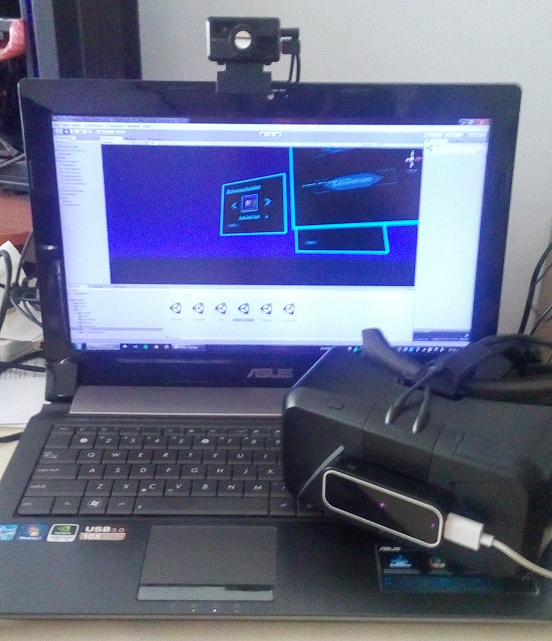
\includegraphics[width=0.75\columnwidth]{images/equipmentpng.png}
\caption{Port\'atil, Dispositivos y Entorno de Desarrollo Empleado}
\label{fig:equipment}
\end{figure}

Para la medición de los recursos computacionales empleados por nuestra solución, se empleó la herramienta Profiler de Unity \cite{PROFILER}, y ejecutándose 30 veces para obtener un promedio. El tiempo de procesamiento de la solución de software en un estado ocioso es de 1.55 ms con un porcentaje de distribución de tiempo balanceado. Sin embargo, los picos más altos de procesamiento se dan en presencia de una gran cantidad de objetos y la interacción del usuario. Así, se llega a alcanzar un tiempo de procesamiento de 32.05 ms con 88.1\% del tiempo consumido por el controlador LeapHand. Este comportamiento se debe a la recolección de basura que ocasiona la versión actual del SDK del dispositivo Leap Motion. Eventualmente se puede presenciar una caída de cps (cuadros por segundo) en la interacción con la aplicación.

\begin{figure*}[htpb!]
\centering
\begin{tabular}{cc}
\subfloat[]{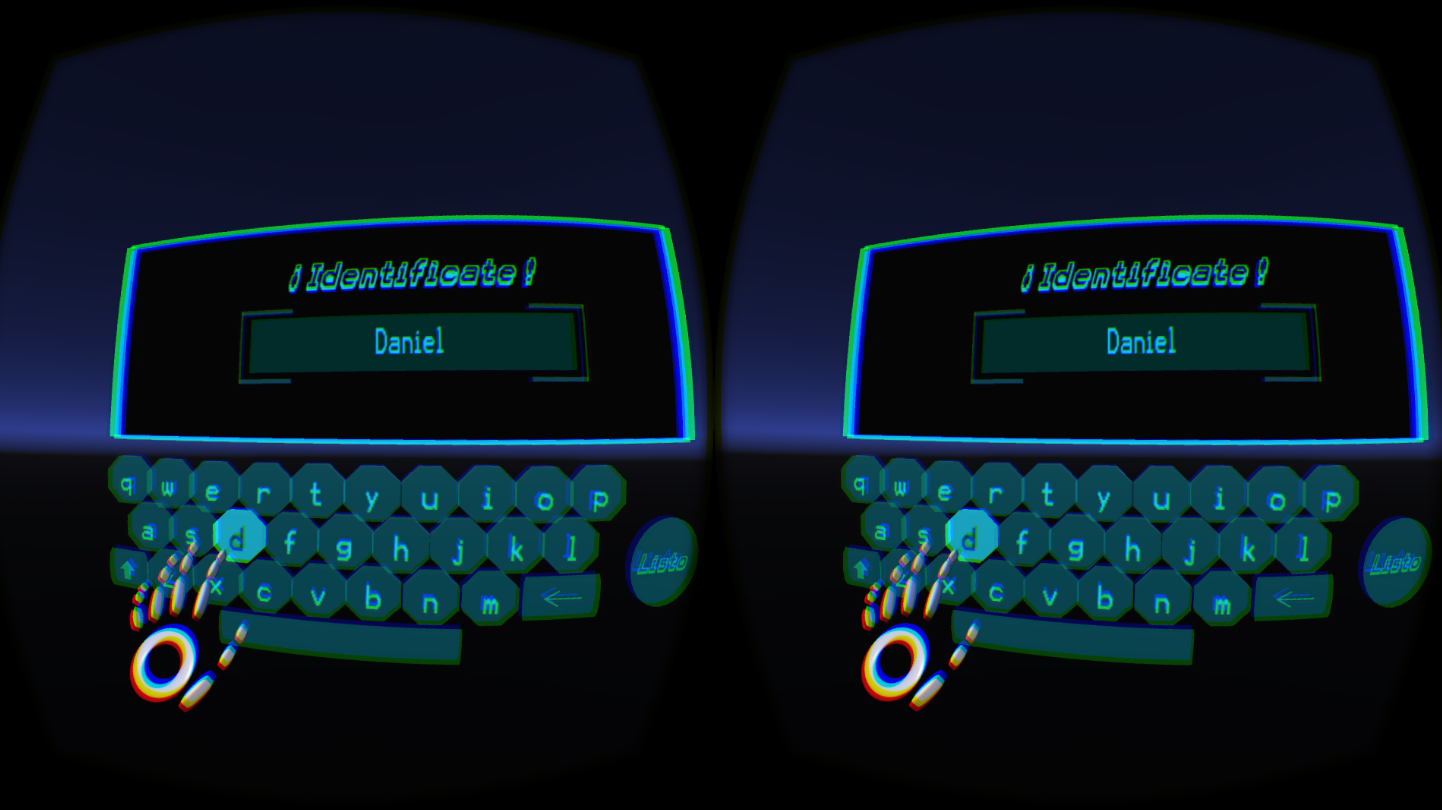
\includegraphics[width=0.49\textwidth]{images/Art1.png}
\label{fig:ux1}
}
\subfloat[]{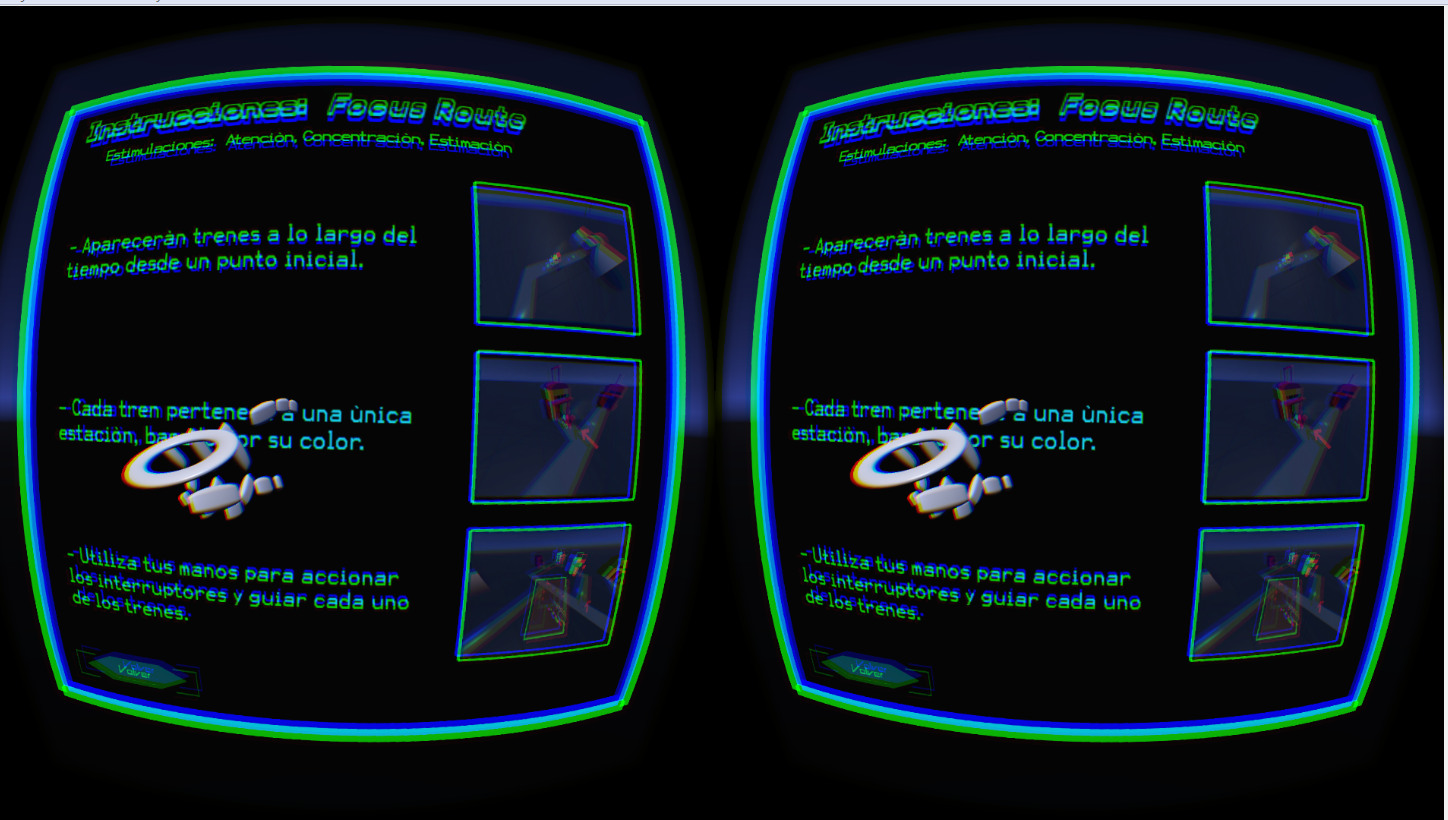
\includegraphics[width=0.49\textwidth]{images/Art4.png}
\label{fig:ux2}
}
\end{tabular}
\caption{Interfaz de Usuario Intuitiva y Gestual Incorporada en Nuestra Solución}
\label{fig:UX}
\end{figure*}

Con respecto a la memoria empleada, debido a la gran cantidad de objetos (estáticos o dinámicos), el consumo de memoria es considerable. En promedio se emplea 0.62 Gb, variando de acuerdo a la cantidad de texturas empleadas en un cuadro visto por el usuario, las animaciones presentes, la cantidad de materiales, entre otros. Si se emplean versiones de menor resolución de los objetos, la cantidad de memoria se reducirá (e.g. algoritmos de reducción de polígonos, niveles de detalle).

Por otro lado, para la evaluación del software se realizó una encuesta a 6 personas con edades comprendidas entre 20-31 años, donde cada uno entrenó con los distintos juegos. Se evaluaron los siguientes criterios: diseño de objetos, jugabilidad y UX. El diseño de objetos representa a la correcta interpretación de los objetos 3D creados, con la representación conocida por el usuario de dicho objeto. La jugabilidad se refiere a la facilidad al realizar de forma satisfactoria el proceso completo de las actividades presentes en cada juego. Por último, UX (experiencia de usuario) indica la experiencia interna de cada persona al interactuar con cada aspecto del juego.

La encuesta se basa en una matriz de lado a lado para el análisis de datos, evaluando importancia/satisfacción (letra \textbf{I} para importancia, y \textbf{S} para satisfacción) para cada uno de los criterios conforme a su respectivo entrenamiento. La escala de varía entre 1-5, donde 1 se considera No Importante/Insatisfecho, y 5 como Importante/Muy Satisfecho. En la Tabla \ref{tb:table1} se muestran los resultados de la encuesta del entrenamiento Ruta de Enfoque. Se puede observar que la jugabilidad es un factor que puede mejorarse en cuanto a la interacción y el posicionamiento del usuario con respecto a panel de control y escenario respectivamente. Sin embargo, el diseño de los objetos y la experiencia de usuario que presenta el entrenamiento es lo suficientemente estable para la satisfacción del usuario.

\begin{table}[htpb!]
\centering
\caption{Resultado de Encuesta para Ruta de Enfoque}
\label{tb:table1}
\begin{tabular}{@{}cc|cc|cc@{}}
\toprule
\multicolumn{2}{c}{Diseño} & \multicolumn{2}{c}{Jugabilidad} & \multicolumn{2}{c}{UX}  \\
\textbf{I}   & \textbf{S}  & \textbf{I}     & \textbf{S}     & \textbf{I} & \textbf{S} \\
4            & 5           & 4              & 4              & 5          & 4          \\
4            & 4           & 4              & 4              & 3          & 4          \\
5            & 4           & 5              & 4              & 5          & 4          \\
3            & 4           & 3              & 3              & 3          & 4          \\
5            & 5           & 5              & 3              & 5          & 5          \\
4            & 4           & 5              & 5              & 4          & 4          \\ \bottomrule
\end{tabular}
\end{table}

La evaluación obtenida para el entrenamiento Paquete de Velocidad se muestra en la Tabla \ref{tb:table2}, donde se hace énfasis en el diseño de los objetos y sus elementos. No obstante, la jugabilidad que presenta se mantiene entre la más valorada en comparación a los otros entrenamientos, teniendo en cuenta que, la experiencia de usuario es un balance entre el diseño y la jugabilidad del mismo.

\begin{table}[htpb!]
\centering
\caption{Resultado de Encuesta para Paquete de Velocidad}
\label{tb:table2}
\begin{tabular}{@{}cc|cc|cc@{}}
\toprule
\multicolumn{2}{c}{Diseño} & \multicolumn{2}{c}{Jugabilidad} & \multicolumn{2}{c}{UX}  \\
\textbf{I}   & \textbf{S}  & \textbf{I}     & \textbf{S}     & \textbf{I} & \textbf{S} \\
5            & 2           & 5              & 5              & 4          & 4          \\
5            & 1           & 4              & 5              & 5          & 3          \\
5            & 3           & 5              & 4              & 4          & 4          \\
4            & 3           & 5              & 5              & 5          & 4          \\
5            & 3           & 5              & 5              & 4          & 3          \\
4            & 4           & 4              & 4              & 5          & 5          \\ \bottomrule
\end{tabular}
\end{table}

Por último, el resultado para el entrenamiento Puntos / Punto se refleja en la Tabla \ref{tb:table3}. Analizando la tabla se puede deducir que una jugabilidad ligeramente insatisfactoria. Según las opiniones recibidas (en retroalimentación obtenida posterior a la encuesta), esto se debe al nivel de dificultad que presenta el entrenamiento en cuanto a la interacción y la modelación de las figuras.

\begin{table}[htpb!]
\centering
\caption{Resultado de Encuesta para Punto / Puntos}
\label{tb:table3}
\begin{tabular}{@{}cc|cc|cc@{}}
\toprule
\multicolumn{2}{c}{Diseño} & \multicolumn{2}{c}{Jugabilidad} & \multicolumn{2}{c}{UX}  \\
\textbf{I}   & \textbf{S}  & \textbf{I}     & \textbf{S}     & \textbf{I} & \textbf{S} \\
4            & 3           & 4              & 3              & 4          & 4          \\
4            & 2           & 4              & 4              & 4          & 4          \\
5            & 3           & 4              & 2              & 4          & 3          \\
5            & 3           & 4              & 3              & 4          & 4          \\
5            & 2           & 5              & 3              & 5          & 4          \\
5            & 3           & 5              & 3              & 4          & 5          \\ \bottomrule
\end{tabular}
\end{table}

En cuanto a la interfaz de usuario, esta fue aceptada por todos los usuarios de forma satisfactoria. De hecho, no se requirió instrucciones extras para los usuarios antes de empezar. En la Figura \ref{fig:UX} se muestran un par de instantes dentro que la solución antes de empezar los juegos que consiste en la introducción de datos \ref{fig:UX}(a), y la selección de los juegos \ref{fig:UX}(b).

% An example of a floating figure using the graphicx package.
% Note that \label must occur AFTER (or within) \caption.
% For figures, \caption should occur after the \includegraphics.
% Note that IEEEtran v1.7 and later has special internal code that
% is designed to preserve the operation of \label within \caption
% even when the captionsoff option is in effect. However, because
% of issues like this, it may be the safest practice to put all your
% \label just after \caption rather than within \caption{}.
%
% Reminder: the "draftcls" or "draftclsnofoot", not "draft", class
% option should be used if it is desired that the figures are to be
% displayed while in draft mode.
%
%\begin{figure}[!t]
%\centering
%\includegraphics[width=2.5in]{myfigure}
% where an .eps filename suffix will be assumed under latex, 
% and a .pdf suffix will be assumed for pdflatex; or what has been declared
% via \DeclareGraphicsExtensions.
%\caption{Simulation results for the network.}
%\label{fig_sim}
%\end{figure}

% Note that the IEEE typically puts floats only at the top, even when this
% results in a large percentage of a column being occupied by floats.


% An example of a double column floating figure using two subfigures.
% (The subfig.sty package must be loaded for this to work.)
% The subfigure \label commands are set within each subfloat command,
% and the \label for the overall figure must come after \caption.
% \hfil is used as a separator to get equal spacing.
% Watch out that the combined width of all the subfigures on a 
% line do not exceed the text width or a line break will occur.
%
%\begin{figure*}[!t]
%\centering
%\subfloat[Case I]{\includegraphics[width=2.5in]{box}%
%\label{fig_first_case}}
%\hfil
%\subfloat[Case II]{\includegraphics[width=2.5in]{box}%
%\label{fig_second_case}}
%\caption{Simulation results for the network.}
%\label{fig_sim}
%\end{figure*}
%
% Note that often IEEE papers with subfigures do not employ subfigure
% captions (using the optional argument to \subfloat[]), but instead will
% reference/describe all of them (a), (b), etc., within the main caption.
% Be aware that for subfig.sty to generate the (a), (b), etc., subfigure
% labels, the optional argument to \subfloat must be present. If a
% subcaption is not desired, just leave its contents blank,
% e.g., \subfloat[].


% An example of a floating table. Note that, for IEEE style tables, the
% \caption command should come BEFORE the table and, given that table
% captions serve much like titles, are usually capitalized except for words
% such as a, an, and, as, at, but, by, for, in, nor, of, on, or, the, to
% and up, which are usually not capitalized unless they are the first or
% last word of the caption. Table text will default to \footnotesize as
% the IEEE normally uses this smaller font for tables.
% The \label must come after \caption as always.
%
%\begin{table}[!t]
%% increase table row spacing, adjust to taste
%\renewcommand{\arraystretch}{1.3}
% if using array.sty, it might be a good idea to tweak the value of
% \extrarowheight as needed to properly center the text within the cells
%\caption{An Example of a Table}
%\label{table_example}
%\centering
%% Some packages, such as MDW tools, offer better commands for making tables
%% than the plain LaTeX2e tabular which is used here.
%\begin{tabular}{|c||c|}
%\hline
%One & Two\\
%\hline
%Three & Four\\
%\hline
%\end{tabular}
%\end{table}


% Note that the IEEE does not put floats in the very first column
% - or typically anywhere on the first page for that matter. Also,
% in-text middle ("here") positioning is typically not used, but it
% is allowed and encouraged for Computer Society conferences (but
% not Computer Society journals). Most IEEE journals/conferences use
% top floats exclusively. 
% Note that, LaTeX2e, unlike IEEE journals/conferences, places
% footnotes above bottom floats. This can be corrected via the
% \fnbelowfloat command of the stfloats package.




\section{Conclusiones} \label{conclusiones}
El estímulo de las áreas cognitivas por medio de entrenamientos mentales a través de juegos adaptados a un ambiente de realidad virtual, se presentó en este artículo. Con la selección del juego, el usuario puede decidir qué áreas cognitivas desea estimular y/o visualizar el desempeño que ha obtenido con los distintos entrenamientos, interactuando por medio de una interfaz natural de usuario. Así, la inteligencia espacial permite al cerebro pensar de forma precisa y lógica la solución de un problema real o imaginario. La práctica constante de ejercicios, tareas o actividades relacionadas a las habilidades espaciales ayuda al cerebro a estimular aquellas áreas cognitivas utilizadas en este tipo de capacidad de pensamiento. 

Los entrenamientos desarrollados basados en la inteligencia espacial permiten al usuario experimentar un entorno de realidad virtual de inmersión total a través de la interacción gestual. Cada dificultad que representa un entrenamiento, modifica las propiedades, los componentes y sus controladores ofreciendo un nuevo nivel de desenvolvimiento con el mismo. Del mismo modo, el proceso estadístico empleado, permite estimar los valores de las distintas estimulaciones cognitivas por medio del tiempo de respuesta que el usuario realice ante una tarea, logrando obtener resultados apropiados y acertados para el control del mismo.

Los resultados obtenidos muestran que el consumo de recursos computacionales es aceptable, considerando el uso de un portátil de prestaciones media. Por otro lado, las encuestas realizadas permiten deducir una aceptación satisfactoria por parte de los usuarios. Sin embargo, es claro que las pruebas no son suficientes (cantidad, aspectos medidos, edades) para obtener resultados concluyentes del impacto del estudio; siendo un buen inicio a investigaciones futuras. Igualmente, podemos estimar que mejorar el hardware (e.g. tarjeta de video de alta generación) o incluir versiones nuevas del software (e.g. SDK de Oculus, versión 5.5+ de Unity3d), pueden influir positivamente en el rendimiento global de la solución. 

En un futuro, se propone construir ambientes virtuales más realistas añadiendo elementos de iluminación global en las escenas como \textit{ambient occlusion}, \textit{color bleeding}, sombras suaves, entre otros. Igualmente, se propone añadir un módulo de ``tutorial en vivo'' que permita indicar al usuario los objetivos del entrenamiento justo antes de iniciarlo, es decir, un escenario similar al entrenamiento seleccionado que contenga una inteligencia artificial indicando las acciones que debe realizar.


% conference papers do not normally have an appendix


% use section* for acknowledgment
%\section*{Agradecimientos}
%The authors would like to thank...
%Este trabajo fue apoyado por los proyectos de Catalu\~na, de Espa\~na y de Europa identificados como DPI2015-65286-R, 2014-SGR-1470 y CERCA Programme / Generalitat de Catalunya.
%This work was supported by Catalan, Spanish and European projects DPI2015-65286-R, 2014-SGR-1470, CERCA Programme / Generalitat de Catalunya. The Titan X  Pascal used for this research was donated by the NVIDIA Corporation.




% trigger a \newpage just before the given reference
% number - used to balance the columns on the last page
% adjust value as needed - may need to be readjusted if
% the document is modified later
%\IEEEtriggeratref{8}
% The "triggered" command can be changed if desired:
%\IEEEtriggercmd{\enlargethispage{-5in}}

% references section

% can use a bibliography generated by BibTeX as a .bbl file
% BibTeX documentation can be easily obtained at:
% http://mirror.ctan.org/biblio/bibtex/contrib/doc/
% The IEEEtran BibTeX style support page is at:
% http://www.michaelshell.org/tex/ieeetran/bibtex/
%\bibliographystyle{IEEEtran}
% argument is your BibTeX string definitions and bibliography database(s)
\balance
\bibliographystyle{IEEEtran}
\bibliography{books} 

%
% <OR> manually copy in the resultant .bbl file
% set second argument of \begin to the number of references
% (used to reserve space for the reference number labels box)



% that's all folks
\end{document}


